% ==============================================================
%  Chapter 4 -- Experimental Study
% ==============================================================

\chapter{Experimental Study}
\label{ch:experiments}

This chapter evaluates the pipeline of Chapter~\ref{ch:implementation} on two real influence diagrams of clinical origin. The
\emph{bypass} diagram, already introduced in
Section~\ref{sec:bypass-example} as the running example of the
implementation, plays the role of a small sanity-check benchmark. The
\emph{NHLy} diagram, presented in the next section, is one order of
magnitude larger and constitutes the main benchmark of the empirical study.

% ==============================================================
\section{Benchmark networks}
\label{sec:benchmarks}
% ==============================================================

The experimental study uses two influence diagrams of clinical origin and very
different size: the small \emph{bypass} diagram, which serves as a controlled
benchmark, and the much larger \emph{NHLy} diagram, which stresses the method on
a realistic parameter vector. This section introduces both.

\subsection{Bypass: management of coronary heart disease}
\label{sec:bypass-bench}

The \emph{bypass} diagram was already presented in
Section~\ref{sec:bypass-example} as the illustrative model used to
explain the implementation. It is reused here as a small, controlled benchmark on which the parameter vector is small enough for a finer study of the encoding, the decoding, the loss and the EDA variant.


\subsection{NHLy: management of non-Hodgkin lymphoma}
\label{sec:nhlv1}

The \emph{NHLy} influence diagram models the clinical management of
gastric non-Hodgkin lymphoma~\cite{boot1998gastric}. Its qualitative structure is shown in
Figure~\ref{fig:nhlv1-id}. It comprises sixteen chance nodes
covering disease, treatment-side-effect and outcome variables, three
decision nodes (\texttt{Surgery}, \texttt{Helicobacter treatment} and
\texttt{CT-RT schedule}) and a single utility node. Because of its
size and connectivity, the parameter vector
$\boldsymbol{\Theta}$ associated with the diagram is of the order of
several thousand entries (Table~\ref{tab:benchmark-sizes}), which makes the elicitation bottleneck
discussed in Chapter~\ref{ch:introduction} fully tangible and the
EDA-based recovery the only practical route to populating the
network.
\\

\begin{table}[h]
\centering
\begin{tabular}{l|rr|r|rr}
\hline
& \multicolumn{2}{c|}{\textbf{CPT entries}} & \textbf{Utility ent.}
& \multicolumn{2}{c}{\textbf{Total} $|\boldsymbol{\Theta}|$}\\
& \multicolumn{1}{c}{all} & \multicolumn{1}{c|}{free} & &
  \multicolumn{1}{c}{all} & \multicolumn{1}{c}{free}\\
\hline
bypass &     86 &    57 &   9 &     95 &     66 \\
NHLy   & 8\,282 & 5\,131 & 144 & 8\,426 & 5\,275 \\
\hline
\end{tabular}
\caption{Size of the parameter vector for the two benchmark networks.
``All'' counts every entry of every CPT row; ``free'' discounts the
one-per-row redundancy introduced by the probabilities constraint
$\sum_j\theta_j=1$.}
\label{tab:benchmark-sizes}
\end{table}

\newpage

To make these parameters concrete, Tables~\ref{tab:nhlv-cpt}
and~\ref{tab:nhlv-util} show, respectively, one real CPT and a slice of the
utility table of \emph{NHLy}; the nodes they involve are marked with an asterisk
in the diagram of Figure~\ref{fig:nhlv1-id}. Table~\ref{tab:nhlv-cpt} gives
$P(\texttt{Perforation}\mid\texttt{CT-RT schedule})$: the risk of perforation
grows monotonically with the aggressiveness of the schedule.
Table~\ref{tab:nhlv-util} shows how the utility depends on the five-year outcome
and the patient's general health status, with the remaining three parents fixed:
survival dominates the value and the health status only modulates it.

\begin{table}[h]
\centering\small
\begin{tabular}{l|cc}
\hline
$P(\texttt{Perforation} \mid \texttt{CT-RT schedule})$ & \textsc{no} & \textsc{yes}\\
\hline
$\texttt{CT-RT} = \textsc{none}$                                 & 0.99 & 0.01\\
$\texttt{CT-RT} = \textsc{radiotherapy}$                         & 0.97 & 0.03\\
$\texttt{CT-RT} = \textsc{chemotherapy}$                         & 0.95 & 0.05\\
$\texttt{CT-RT} = \textsc{chemo}\!\rightarrow\!\textsc{radio}$   & 0.92 & 0.08\\
\hline
\end{tabular}
\caption{A real CPT of \emph{NHLy}: probability of \texttt{Perforation}
conditioned on the \texttt{CT-RT schedule}. Each row is a probability
distribution over the two outcomes. The two nodes involved are starred ($^{\ast}$)
in Figure~\ref{fig:nhlv1-id}.}
\label{tab:nhlv-cpt}
\end{table}

\begin{table}[h]
\centering\small
\begin{tabular}{l|ccc}
\hline
\multicolumn{4}{l}{$u(\texttt{FiveYearResult},\ \texttt{GeneralHealthStatus})$}\\
\multicolumn{4}{l}
 {\footnotesize(parents fixed:
\footnotesize\texttt{HelicobacterTreatment}=\textsc{no},\ \
\texttt{Surgery}=\textsc{none},\ \ \texttt{CT-RT}=\textsc{none})}\\
\hline
                                           & \textsc{poor} & \textsc{average} & \textsc{good}\\
\hline
$\texttt{FiveYearResult} = \textsc{alive}$ & 0.90 & 0.95 & 1.00\\
$\texttt{FiveYearResult} = \textsc{death}$ & 0.15 & 0.18 & 0.25\\
\hline
\end{tabular}
\caption{A slice of the \emph{NHLy} utility table (which has $144$ entries over
five parents). Three parents are held fixed and the value is shown as a function
of the five-year result and the general health status: survival dominates the
utility and the health status only modulates it. The nodes involved are starred
($^{\ast}$) in Figure~\ref{fig:nhlv1-id}.}
\label{tab:nhlv-util}
\end{table}

The Influence Diagram illustrated in Figure~\ref{fig:nhlv1-id} models a complex medical treatment process, involving three sequential decisions: \texttt{Helicobacter Treatment}, \texttt{Surgery}, and \texttt{CT RT Schedule} (chemotherapy and radiotherapy). 

Unlike simpler diagnostic models, this diagram captures a broad spectrum of clinical chance variables. These encompass the patient's baseline profile (such as \texttt{Age}, \texttt{General Health Status}, and \texttt{Clinical Stage}), intermediate physiological res$-$ \\ponses and severe complications (like \texttt{Hemorrhage}, \texttt{BM Depression}, or \texttt{Perforation}), and various survival metrics across different treatment stages. 

Ultimately, the overall clinical preference is captured by a single \emph{Utility} node that evaluates the consequences of the entire chosen clinical pathway, culminating in long-term assessments such as the \texttt{Five Year Result}.


\begin{landscape}
\begin{figure}[p]
\centering
\begin{tikzpicture}[
    x=1.35cm, y=1.25cm, % Amplía el espacio entre nodos para evitar solapamientos
    every node/.style={font=\sffamily\scriptsize, align=center, inner sep=2pt},
    chance/.style={ellipse, draw=blue!50, fill=cyan!15,
                   minimum width=2.2cm, minimum height=0.9cm},
    decision/.style={rectangle, draw=black, fill=orange!30,
                     minimum width=2.2cm, minimum height=1.0cm},
    utility/.style={regular polygon, regular polygon sides=6,
                    shape border rotate=90,
                    draw=black, fill=purple!30,
                    minimum width=2.4cm, minimum height=1.0cm, inner sep=2pt},
    arr/.style={-{Stealth[scale=1.0]}, draw=blue!60!black},
    info/.style={-{Stealth[scale=1.0]}, draw=blue!60!black, dashed}
]
    % ==========================================
    %  Posición de Nodos (Ajustados al Layout)
    % ==========================================

    %  --- Fuentes / observaciones ---
    \node[chance]   (AGE)    at ( 0, 10)   {AGE};
    \node[chance]   (GHS)    at ( 0,  6)   {GENERAL HEALTH\\STATUS\,$^{\ast}$};
    \node[chance]   (HPYL)   at ( 0, -1)   {HELICOBACTER\\PYLORI};

    %  --- Decisiones ---
    \node[decision] (SURG)   at ( 3.5,  5)   {SURGERY};
    \node[decision] (HTRT)   at ( 2,  1)   {HELICOBACTER\\TREATMENT};
    \node[decision] (CTRT)   at ( 4, 10)   {CT RT\\SCHEDULE\,$^{\ast}$};

    %  --- Erradicación ---
    \node[chance]   (ERAD)   at ( 3, -1)   {ERADICATION};

    %  --- Cadena Quirúrgica y Clínica ---
    \node[chance]   (PSRV)   at ( 6,  7.5) {POST SURGICAL\\SURVIVAL};
    \node[chance]   (CLIN)   at ( 6,  4)   {CLINICAL\\PRESENTATION};
    \node[utility]  (UTIL)   at ( 6,  1.5) {UTILITY\,$^{\ast}$};
    \node[chance]   (HIST)   at ( 6, -1)   {HISTOLOGICAL\\CLASSIFICATION};

    %  --- Cadena CT-RT ---
    \node[chance]   (HEM)    at ( 9, 10)   {HEMORRHAGE};
    \node[chance]   (BM)     at ( 8,  9)   {BM DEPRESSION};
    \node[chance]   (BULKY)  at ( 9.5,  3)   {BULKY DISEASE};

    \node[chance]   (IMM)    at (8,  6)   {IMMEDIATE\\SURVIVAL};
    \node[chance]   (POCT)   at (11,  8)   {POST CT RT\\SURVIVAL};
    \node[chance]   (CSTG)   at (11, 0)   {CLINICAL STAGE};

    \node[chance]   (PERF)   at (13,  6)   {PERFORATION\,$^{\ast}$};
    \node[chance]   (THER)   at (13, 10)   {THERAPY\\ADJUSTMENT};

    %  --- Endpoints ---
    \node[chance]   (EARLY)  at (15,  4)   {EARLY RESULT};
    \node[chance]   (FIVE)   at (15,  0)   {FIVE YEAR\\RESULT\,$^{\ast}$};


    % ==========================================
    %  Arcos (Totalmente Rectos)
    % ==========================================
    
    %  AGE -> ...
    \draw[arr] (AGE) -- (GHS);
    \draw[arr] (AGE) -- (BM);
    \draw[arr] (AGE) -- (HIST);
    \draw[arr] (AGE) -- (CSTG);
    \draw[arr] (AGE) -- (BULKY);
    \draw[arr] (AGE) -- (FIVE);

    %  GHS / CLIN / SURG -> PSRV
    \draw[arr] (GHS)  -- (PSRV);
    \draw[arr] (CLIN) -- (PSRV);
    \draw[arr] (SURG) -- (PSRV);

    %  CTRT -> ...
    \draw[arr] (CTRT) -- (HEM);
    \draw[arr] (CTRT) -- (BM);
    \draw[arr] (CTRT) -- (PERF);
    \draw[arr] (CTRT) -- (EARLY);

    %  Complicaciones -> THER / POCT
    \draw[arr] (BM)   -- (THER);
    \draw[arr] (HEM)  -- (THER);
    \draw[arr] (PERF) -- (THER);
    \draw[arr] (HEM)  -- (POCT);
    \draw[arr] (PERF) -- (POCT);

    %  Survival chain
    \draw[arr] (POCT) -- (IMM);
    \draw[arr] (PSRV) -- (IMM);

    %  Surgery / decisions -> outcomes
    \draw[arr] (SURG) -- (EARLY);
    \draw[arr] (THER) -- (EARLY);

    %  HTRT chain
    \draw[arr] (HPYL) -- (ERAD);
    \draw[arr] (HTRT) -- (ERAD);
    \draw[arr] (ERAD) -- (EARLY);

    %  Classification / staging -> outcomes
    \draw[arr] (HIST) -- (BULKY);
    \draw[arr] (CSTG) -- (BULKY);
    \draw[arr] (BULKY) -- (EARLY);
    \draw[arr] (HIST) -- (EARLY);
    \draw[arr] (CSTG) -- (EARLY);

    %  EARLY -> FIVE and parents of FIVE
    \draw[arr] (EARLY) -- (FIVE);
    \draw[arr] (CSTG)  -- (FIVE);
    \draw[arr] (BULKY) -- (FIVE);
    \draw[arr] (HIST)  -- (FIVE);
    \draw[arr] (IMM)   -- (FIVE);

    %  Utility parents
    \draw[arr] (HTRT) -- (UTIL);
    \draw[arr] (SURG) -- (UTIL);
    \draw[arr] (CTRT) -- (UTIL);
    \draw[arr] (GHS)  -- (UTIL);
    \draw[arr] (FIVE) -- (UTIL);


    % ==========================================
    %  Arcos informacionales (Líneas Discontinuas)
    % ==========================================
    
    %  Hacia HTRT
    \draw[info] (HPYL)  -- (HTRT);
    \draw[info] (CSTG)  -- (HTRT);
    \draw[info] (HIST)  -- (HTRT);
    \draw[info] (BULKY) -- (HTRT);
    
    %  Hacia SURG
    \draw[info] (GHS)  -- (SURG);
    \draw[info] (CLIN) -- (SURG);
    \draw[info] (HTRT) -- (SURG);
    
    %  Hacia CTRT
    \draw[info] (SURG) -- (CTRT);

\end{tikzpicture}
\caption{Influence diagram of the \emph{NHLy} model for the management of gastric non-Hodgkin lymphoma. Nodes marked with an asterisk ($^{\ast}$) are those involved in the example CPT and utility slice of Tables~\ref{tab:nhlv-cpt} and~\ref{tab:nhlv-util}.}
\label{fig:nhlv1-id}
\end{figure}
\end{landscape}


% ==============================================================
\section{Experimental protocol}
\label{sec:protocol}
% ==============================================================

The goal of the recovery is operational: to reproduce the
\emph{decisions} the expert would take. Everything in this chapter is
measured towards that goal. As mentioned previously, the rule bases are \emph{synthetic}
(generated by evaluating the original diagram, as described in
Chapter~\ref{ch:implementation}) and then, the ground-truth model is known, so
the recovery can be judged quantitatively.

Here, several important qualifications must be made. Not all recovered models are equally informative: rule bases do not fully determine every component of an influence diagram (solution space is highly degenerated), and different recovery methods vary in their ability to reconstruct the underlying model depending on the initialization and the given rules. Consequently, this dictates the hierarchy of the metrics below.

\subsection{Experiment metrics}
\label{sec:metrics}

Each run is summarised by a small set of quantities, ordered here by how
much they matter for the recovery problem. They are computed on the
\emph{satisfiers} of a run --- the individuals that reproduce the training rules
--- by taking their mean, and aggregated over the independent repetitions with different rules and random initialization.

\begin{enumerate}
  \item \textbf{Rule accuracy (the primary measure).} The fraction of the
        \emph{whole} rule base that the recovered policy reproduces (equivalently $1-\mathcal{L}$ for the $0$--$1$ loss of
        Definition~\ref{def:cost}). Reproducing the expert's decisions is the actual objective, and in a real elicitation it is the only signal available. We report its \textbf{mean} over the
        repetitions.
  \item \textbf{Dispersion of the accuracy (reliability).} EDAs are stochastic methods; therefore, their quality depends not only on their performance but also on their repeatability and robustness to variations in the rule base and parameter initialization: one
        that swings between $80\%$ and $100\%$ across seeds is worse than
        one that sits steadily at $95\%$. We therefore report the
        \textbf{standard deviation} of the accuracy alongside its mean.
  \item \textbf{Recovery time (cost).} How expensive it is to reach that
        accuracy: the number of generations to convergence and the CPU
        time, measured as process CPU seconds rather
        than wall-clock, so that optimizers (EDAs) with very different
        per-generation cost are compared fairly. This metric becomes particularly important for large models, where recovery time can increase dramatically with the number of parameters.

        
  \item \textbf{Probability reconstruction (a secondary objective).} The
        mean squared error of the recovered conditional probability
        tables against the ground truth, $\mathrm{MSE}_{\text{CPT}}$.
        Unlike the rules, this rewards recovering the \emph{actual}
        probabilities, which are objective quantities with a true target;
        doing so is a stronger, desirable outcome, but it is subordinate
        to reproducing the rules and only meaningful where the chance
        model is itself optimized (in most experiments with NHLy, only utilities will be recovered, leaving appart probabilities, to reduce the computational cost).
%   \item \textbf{Utility distance (a diagnostic only, never a score).} The
%         distance between the recovered and the true utility is
%         \emph{not} used to rank anything. The optimal policy is invariant
%         under any transformation of the utility that preserves the
%         $\arg\max$ of the expected utility --- a positive affine rescaling
%         and, more generally, the whole region in which no decision flips
%         --- so infinitely many utility vectors reproduce exactly the same
%         rules. A perfectly correct recovery can thus sit arbitrarily far
%         from the ground-truth numbers. We report this distance only to
%         \emph{illustrate} the degeneracy of
%         Chapter~\ref{ch:framework}, never as a measure of quality.
\end{enumerate}

The ordering is deliberate. Quality is judged first by \emph{how many
rules} are reproduced and \emph{how reliably}, then by \emph{how
cheaply}; recovering the probability tables is a welcome bonus.
% ; and the
% utility numbers are explicitly removed from the scoreboard because the
% problem does not identify them.

\subsection{Several repetitions}
\label{sec:repetitions}

An EDA recovery is stochastic in two distinct ways, so a single run is a sample
of a random variable rather than a fixed measurement:
\begin{itemize}
  \item \textbf{The optimizer is itself randomized:} it starts from a random
        initial model (individuals drawn from a uniform distribution) and at each
        generation re-estimates the model from the highest-accuracy subset of the
        population before sampling the next one, so even on the very same rules
        two runs may follow different trajectories and may settle on different
        policies (as Section~\ref{sec:stopmode} examines in detail).
  \item \textbf{Which rules are exposed is itself a random draw:} each run trains
        on a given fraction of the rule base, and the particular subset of
        decision rules shown changes what can be identified, since different
        subsets constrain the policy to different degrees.
\end{itemize}
Reporting a single run would therefore conflate
the quality of a method with the luck of one seed. To turn the metrics of
Section~\ref{sec:metrics} into meaningful estimates, we run every configuration
several independent times, each with a different random seed that simultaneously
redraws the initialization and the rule sample: the \textbf{mean} over
repetitions estimates the expected accuracy (the primary metric) and their
\textbf{standard deviation} estimates the reliability (the second metric),
neither of which is computable from a single run.

It is worth noting that, in a real-world application, it would be the expert who
decides which rules to prioritize, according to their importance and how well
they capture the most critical decisions.

\subsection{Loss functions under study}
\label{sec:losses}

The recovery minimizes the aggregated per-rule loss of
Definition~\ref{def:fitness}; the experiments in this chapter sweep its five
instances, which differ only in \emph{how} they penalize for each rule the candidate
gets wrong. They are not redundant, they shape the different strategies, and the purpose of comparing them is to find out whether a
smoother, more informative signal helps the EDA to converge. Briefly:

\begin{itemize}
  \item \textbf{\texttt{binary}} (the $0$--$1$ loss). Counts how many training
        rules the candidate fails to reproduce, scoring nothing for
        \emph{how} wrong each one is. It is the strictest criterion and the one that most faithfully reflects the actual objective (rule accuracy), but it yields a loss landscape with many flat regions, which can make it more difficult to converge to local optima. We test it as the natural baseline and the one all
        other losses must beat to be worth their extra complexity.
  \item \textbf{\texttt{regret}} and \textbf{\texttt{margin}}. Instead of a
        yes/no verdict they measure \emph{by how much} the utility of the
        chosen action falls short of the best one, turning the landscape
        continuous and giving the optimizer a direction to descend; \texttt{margin}
        additionally demands a safety gap, rewarding decisions that win
        \emph{clearly} rather than by a little. We test them to see whether this
        smoother signal accelerates or stabilizes
        convergence relative to \texttt{binary}.
  \item \textbf{\texttt{softmax}} and \textbf{\texttt{entropy}}. These score the
        log-likelihood of the expert action under a softmax over the candidate
        utilities; \texttt{entropy}
        adds a regularizer that discourages over-confident utility vectors. We
        test them to check whether the confidence level improves the recovered model.
\end{itemize}

All five will later be crossed against the optimizers; the preliminary study below will fix \texttt{binary} because it is the simplest and the easiest to evaluate.


% ==============================================================
\section{Convergence and the stopping criterion}
\label{sec:stopmode}
% ==============================================================

Prior to conducting a full sweep of the hyperparameter and configuration grid, we performed a couple of preliminary studies. This first study aims to solve, or at least hint at the solutions for, two linked questions that are kept fixed throughout the grid: \emph{when a run should stop}, and \emph{what does converge mean} in the context of a recovery problem.

With the \texttt{binary} fitness, an individual computes 0 penalty score when it reproduces \emph{every} training rule it was shown; we call such individuals \textbf{satisfiers}. A natural stopping rule
is therefore to wait until a given fraction of the population has become a
satisfier: the \texttt{top}$X$ criterion interrupts the run once $X\%$ of the
individuals satisfy all the training rules. We track the thresholds
$X\in\{50,70,90,95,100\}$ together with the four EDA variants (UMDA, EMNA, EGNA
and KEDA on \emph{bypass}; only the cheap UMDA and EMNA on the
\emph{NHLy}, where the multivariate EGNA and the kernel-based KEDA are
too expensive for this preliminary study) and the \texttt{binary}
fitness, exposing $5$, $10$, $20$ and $30\%$ of the decision-rule base. 

The two
benchmarks differ in what is recovered and in how many rules those percentages represent. Besides, on \emph{bypass} the recovery optimizes \emph{both} the conditional
probability tables and the utilities (\texttt{both} mode) and each configuration is repeated $10$ times; its rule base has $20$ decision rules, so the four fractions correspond to $1$, $2$, $4$ and $6$ rules. On \emph{NHLy}, whose size makes a full recovery expensive, \emph{only} the utilities are
optimized (\texttt{utility\_only} mode, leaving the probability tables
untouched) and each configuration is repeated $5$ times; its $67$ decision
rules turn the same fractions into $3$, $7$, $13$ and $20$ rules.

Each run is
capped at $100$ generations with at least $50$ so that the convergence curves
show enough evolution, and each repetition draws a fresh random rule sample and
initialization (different $\texttt{seed}$ in random function).

The crucial point is that satisfying the training rules does \emph{not} fix the complete optimal policy. Many individuals achieve a perfect, zero-loss, fit to the
rules they were shown and yet disagree on the rules they were
\emph{not} shown (due to the degeneracy explained in
Chapter~\ref{ch:framework}). To expose it we measure their accuracy on the \textbf{whole} rule base, and report its mean and its standard deviation across the repetitions.

\subsection{The stabilization level}
\label{sec:stopmode-init}

Figure~\ref{fig:stopmode-reps} shows ten repetitions of a single
configuration (UMDA, \texttt{binary}, $30\%$ of the rules) together with their
mean. \textbf{Every repetition stabilizes} (as the nature of an EDA guarantees):
after the first generations each trajectory reaches a plateau and stays on it,
so the method is well behaved on all seeds. What changes from one run to another
is not \emph{whether} it settles but the \emph{level} at which it does. In this
particular configuration most repetitions stabilize on a $75$--$85\%$ plateau,
but at least one settles much lower, around $50\%$ (not a failure to
converge, but convergence to a policy no better than the one obtained with no
rules at all) so the across-repetition mean sits around $72\%$, below the
better individual runs.

Because each repetition starts from a different random
initialization and sees a different rule sample, \textbf{the outcome of a single
run is itself a random variable}: the same optimizer, fitness and rule budget
can stabilize on a good policy or on a mediocre one depending only on where it
started. The markers \texttt{top50}/\texttt{70}/\texttt{90}/\texttt{95}/\texttt{100}
on the mean curve give the median generation at which each stopping threshold is
reached; that they cluster within a narrow band of generations already
anticipates the next result.


\begin{figure}[h]
\centering
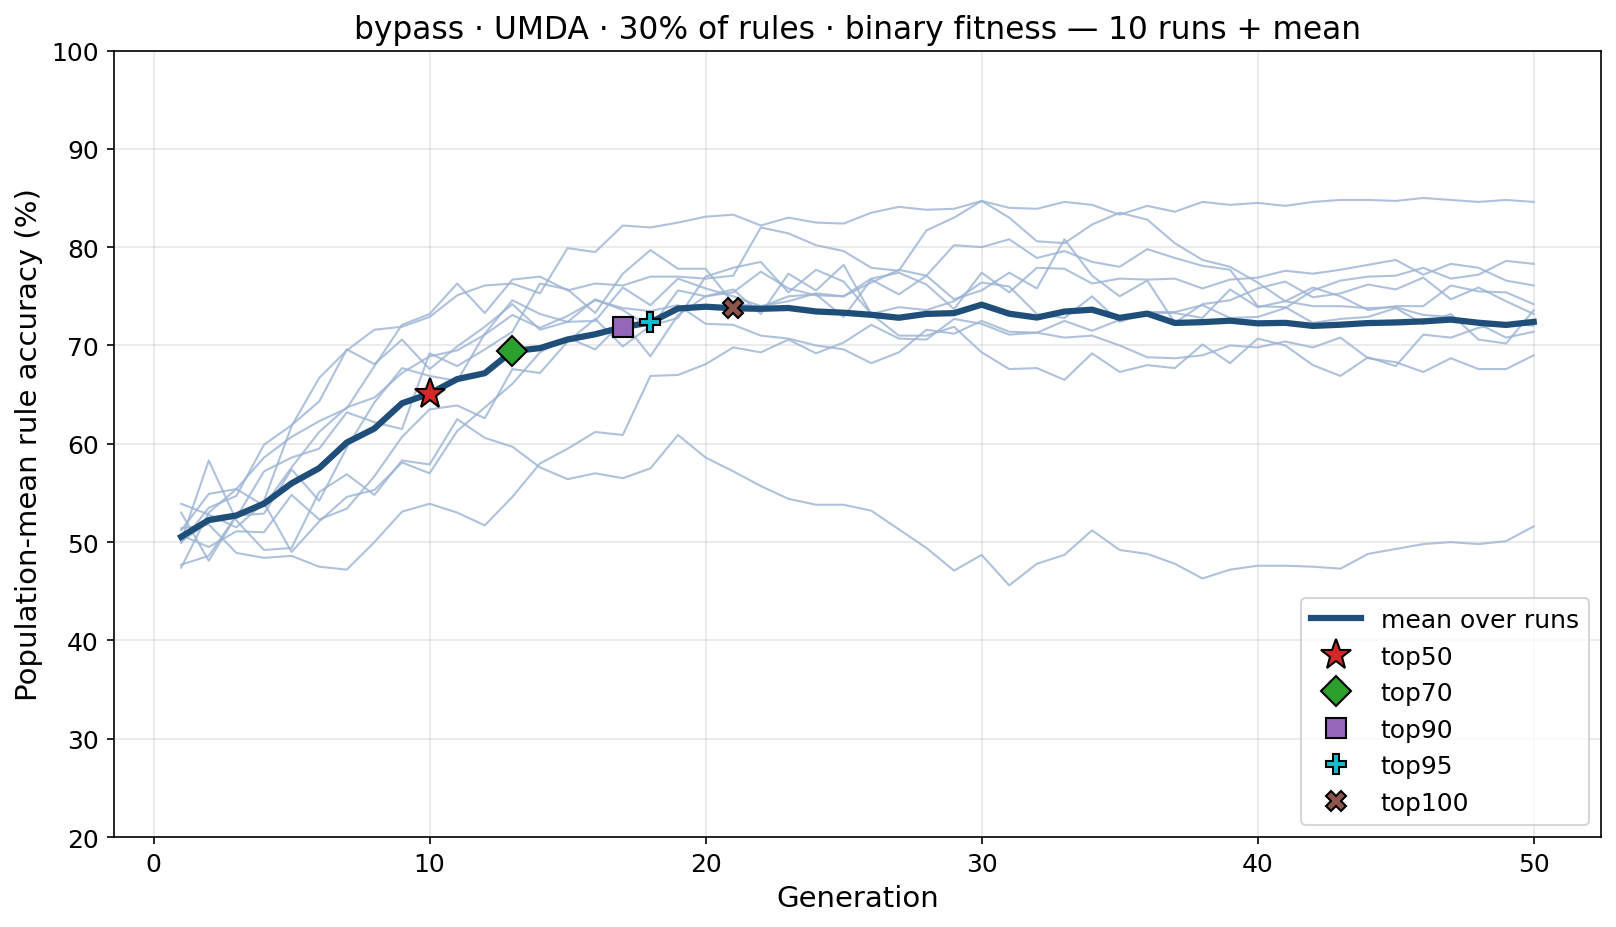
\includegraphics[width=0.95\textwidth]{figures/stopmode_reps_init.png}
\caption{Ten repetitions of a single configuration on \emph{bypass} (UMDA,
\texttt{binary}, $30\%$ of the rules). Thin curves: individual repetitions,
each with its own random initialization and rule sample. Thick curve:
across-repetition mean. The markers
\texttt{topX} indicate the median generation at which the corresponding stopping threshold is reached.}
\label{fig:stopmode-reps}
\end{figure}

\subsection{The stopping threshold: accuracy versus cost}
\label{sec:stopmode-cost}

The stopping criterion controls \emph{when} to stop, and therefore also the cost of a run. It does not change \emph{what} the search does (with a fixed seed the
EDA visits the same sequence of populations). The question then is
purely one of trade-off: \emph{how much accuracy a later stop will yield the extra generations it costs}. Figure~\ref{fig:stopmode-ex-nhlv1} makes it visible
on one \emph{NHLy} configuration. 

Convergence is slow, so the curve keeps climbing well beyond \texttt{top50}: a stricter threshold genuinely buys accuracy, but every increment
costs many generations of an already expensive run, and the strictest thresholds are often \emph{never reached} within a reasonable budget (the \texttt{top100} marker is
absent). A single configuration cannot fix the criterion, though; the trade-off has to be read across all of them at once.

Figure~\ref{fig:stopmode-tradeoff} does exactly that. Setting the threshold
from $10\%$ to $100\%$ and averaging over every optimizer, rule fraction and
repetition, it plots the recovered accuracy against the cost (generations) at
which each threshold would fire.
The curve has a very clear shape on both IDs: accuracy climbs fast,
bends at a knee, then grows significantly slower. \textbf{We adopt \texttt{top90}} as that knee (the threshold that captures essentially all the achievable accuracy while remaining attainable within a reasonable budget.


Going further is a not worth enough: \texttt{top95} and
\texttt{top100} add at most a point before flattening, while the cost climbs from $\sim\!14$ to $\sim\!25$
generations, and \texttt{top100} is reached in only about two-thirds of the runs
($66\%$ on \emph{bypass}, $60\%$ on \emph{NHLy}).
Stopping earlier (\texttt{top50}) would instead forgo
several points specially on \emph{NHLy}. \texttt{top90} is thus the
strictest threshold that is still robustly reachable and we fix it for the rest of the study.

\begin{figure}[h!]
\centering
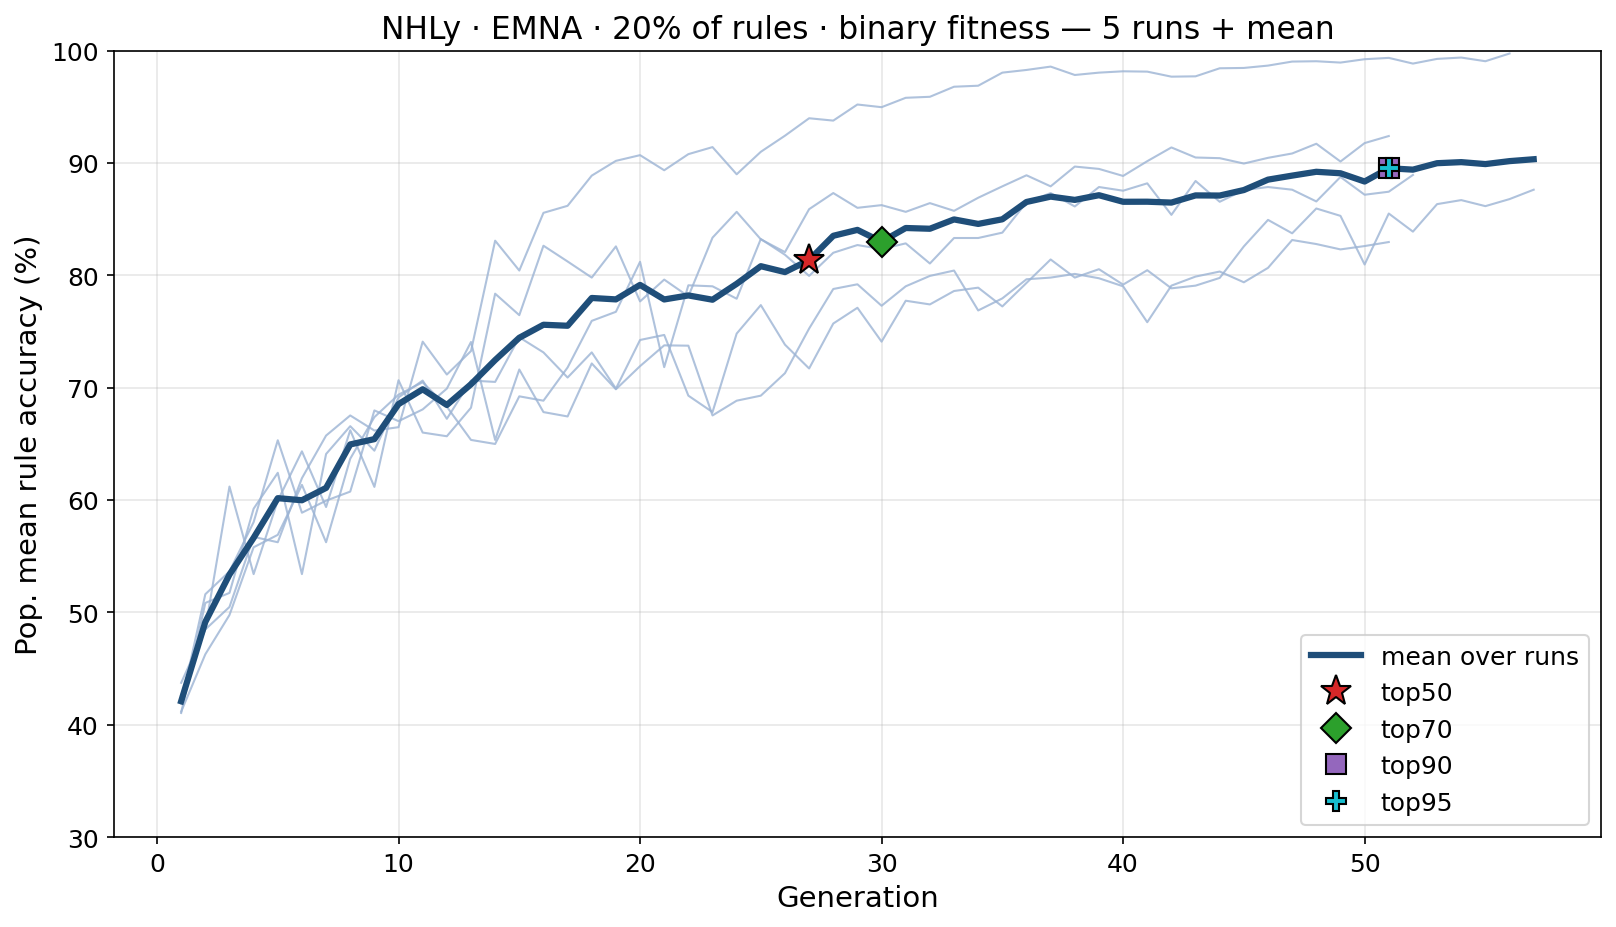
\includegraphics[width=.85\textwidth]{figures/stopmode_example_nhlv1.png}
\caption{Convergence of (\emph{NHLy}, EMNA, \texttt{binary}, $20\%$ of the rules)  configuration; same conventions as Figure~\ref{fig:stopmode-reps}.
Convergence is slower (still rising at \texttt{top50}).}
\label{fig:stopmode-ex-nhlv1}
\end{figure}

\begin{figure}[h!]
\centering
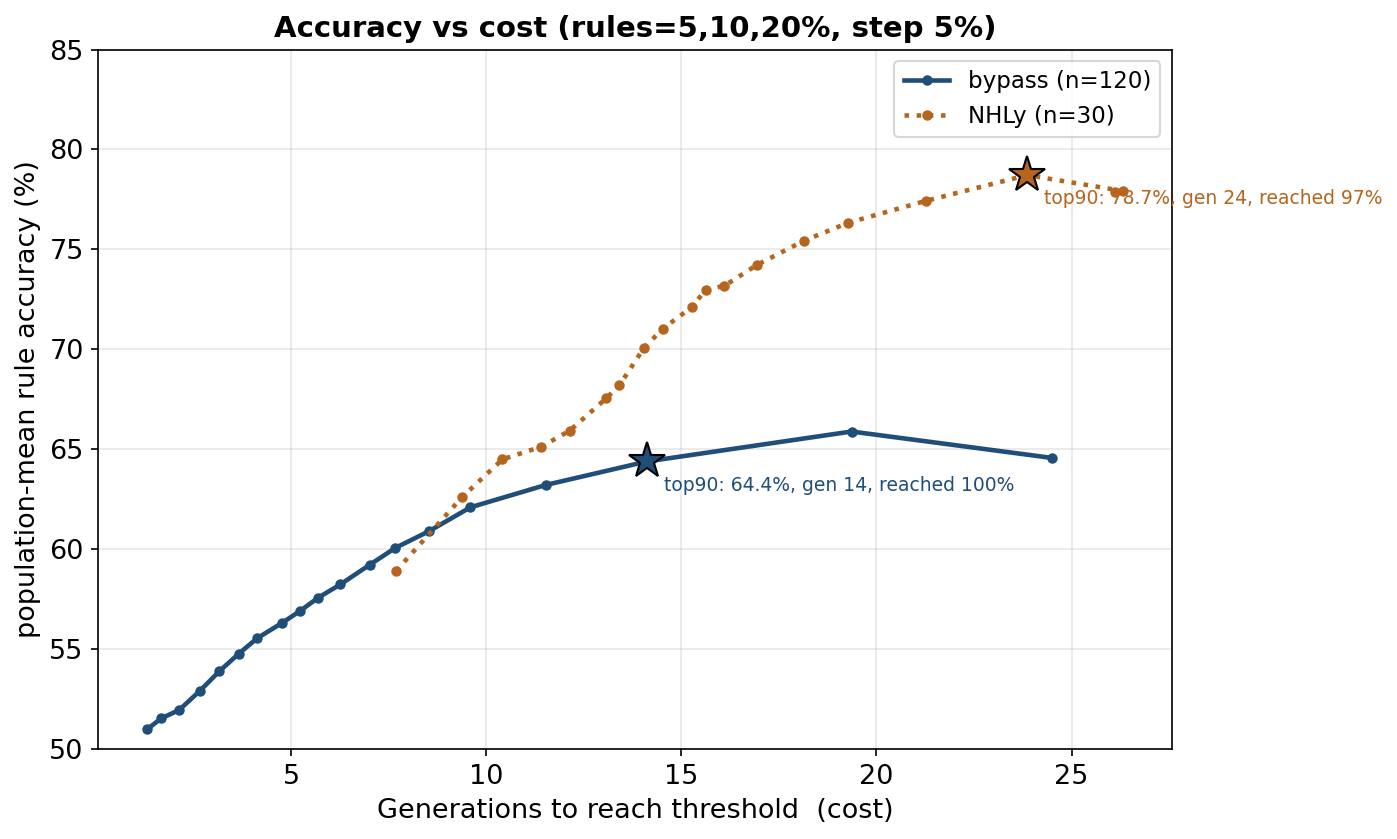
\includegraphics[width=.85\textwidth]{figures/stopmode_tradeoff.png}
\caption{Accuracy versus cost as the stopping threshold sweeps $10\%\to100\%$ in
steps of $5\%$, averaged over every optimizer and repetition for $5$, $10$ and
$20\%$ of the rules (population-mean rule accuracy, \texttt{binary} fitness). The
$x$ axis is the generation at which each threshold fires, its cost. The stars
mark the adopted \texttt{top90} and report its accuracy, cost and how often it is
reached.}
\label{fig:stopmode-tradeoff}
\end{figure}

Two reasons allow us to reuse this single criterion throughout all the experiments, even across completely different configurations such as varying loss functions. 

\begin{itemize}
    \item First, \texttt{top90} is not tied to the \texttt{binary} notion of a satisfier. Instead, it triggers when ``the best $90\%$ of the population reach the \emph{target quality} of the loss in use''. This target is defined per loss function (e.g., zero penalty for \texttt{binary}, the prescribed margin for \texttt{regret}/\texttt{margin}, and the corresponding log-likelihood threshold for \texttt{softmax}/\texttt{entropy}, as detailed later). 

    \item Second, the fitness curve shape that justifies this choice (a steep rise followed by a plateau) is an inherent property of the \emph{EDA dynamics} on this kind of problem, rather than an artifact of any particular loss function. Although the length and steepness of this curve may vary, the loss merely reshapes the landscape that the search algorithm climbs.
\end{itemize}




\newpage


% ==============================================================
\section{Population size of the EDA search}
\label{sec:popsize}
% ==============================================================

Before moving to the main results, we must fix one last parameter: the \textbf{EDA population size}. This is crucial because it determines \emph{how reproducible} a single run is, rather than \emph{whether} it succeeds. 

To set this, we conduct a variance study on \emph{bypass} (\texttt{both}) and \emph{NHLy} (\texttt{utility\_only}). We sweep the population size across several sizes. For each size, we run a full grid of combinations: 5 rule subsets $\times$ 5 initialization seeds over the 5 losses.

Because the rule sample and the population initialization are driven by \emph{independent} seeds, the accuracy variance splits into two components (each caused by a separate stochastic draw): the \textbf{rule effect} (how much the result
moves when the elicited rules change) and the \textbf{init effect} (how much it
moves when only the random initialization of the parameter vector changes).

\subsection{Larger population yields stability, not accuracy}
\label{sec:popsize-stability}

Looking at the \emph{bypass} sweep along the cost axis (Figure~\ref{fig:pop-tradeoff},
right panel) mean accuracy remains \emph{flat}: it sits at
$\sim\!67$--$72\%$ for UMDA/EMNA/EGNA and $\sim\!78$--$80\%$ for KEDA almost regardless of the
population, so a larger population does \emph{not} recover a better policy. What the
population changes is the \emph{dispersion} (left panel). The \textbf{init effect falls
sharply} as the number of individuals grow. At the same time the \textbf{rule variance stays roughly flat} ($\sim\!2$--$3$ points) throughout the sweep.

This is
the central finding of the section: the population suppresses the spread that comes from
the stochastic initialization of the optimizer, but it has a weaker effect on the variance that comes from
\emph{which questions the expert is asked}, which depends on the data input, not of the
search. EMNA is the exception its init effect barely falls (it stays around $3$
points even at $400$), a structural instability the population in not solve (and the
cost, of course, rises with the population).

On \emph{bypass}, a cheap network of seconds
per run, the init effect for UMDA does not improve up to $200$ (it is still
$\sim\!3.4$, as at $50$) and only collapses at $\mathbf{400}$ ($\sim\!1.1$); pushing on
to $800$ buys a marginal $0.2$ point for double the cost. We have chosen $400$ as it provides a good trade-off, and that is the population we adopt for \emph{bypass} throughout the rest of the chapter.

\begin{figure}[h!]
\centering
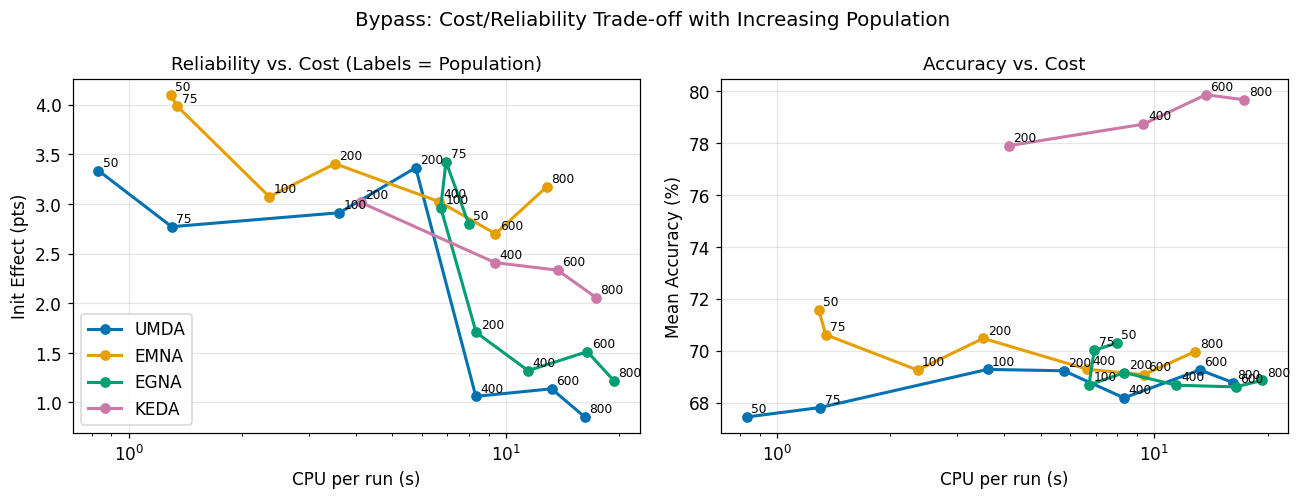
\includegraphics[width=\textwidth]{figures/43_pop_tradeoff.png}
\caption{\emph{Bypass} (\texttt{both}): init effect (left) and mean accuracy (right)
against CPU cost per run, with the population labeling each point.}
\label{fig:pop-tradeoff}
\end{figure}

\subsection{The population drains the init variance, not the rule variance}
\label{sec:popsize-decomp}

The flat rule effect and the collapsing init effect can be read directly by plotting one
component against the other (Figure~\ref{fig:pop-diag-bypass}).
Points above the diagonal are configurations where the initialization dominates the
result; points below are where the drawn rules dominate. At population $100$ most
configurations sit \emph{above} the diagonal: the initialization is still the larger
source of variance. At a population of $400$, the same points have dropped \emph{below} the diagonal (the init. variance is reduced to $\sim\!1$ point, while the rule variance remains unchanged at $\sim\!2$--$3$), leaving only the irreducible sensitivity to the rule sample. This is precisely the behavior anticipated in the previous section, providing strong justification for selecting a population of $400$ for the \emph{bypass} model. Ultimately, we set a population size where the spread introduced by the initialization becomes negligible compared to the inherent variance of the data.

\begin{figure}[h!]
\centering
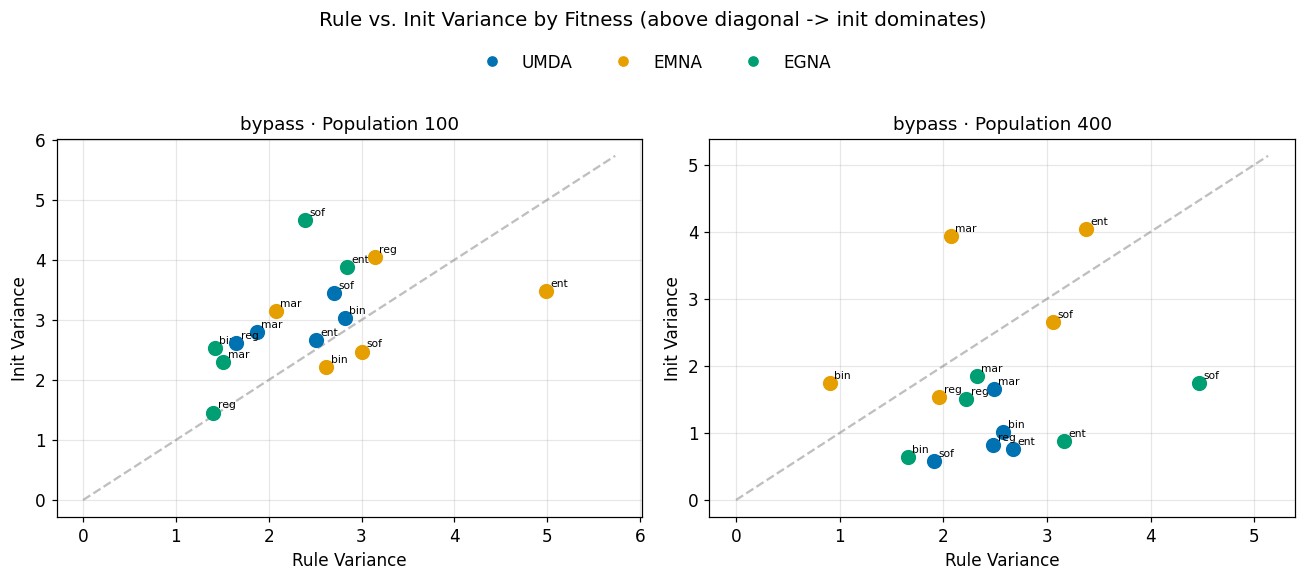
\includegraphics[width=\textwidth]{figures/43_diag_bypass.png}
\caption{\emph{Bypass}: rule effect versus init effect per fitness and optimizer, at
population $100$ (left) and $400$ (right). Above the diagonal the initialization
dominates; below it the drawn rules do. Growing the population from $100$ to $400$ moves
the cloud from above to below the diagonal. The init variance is drained, the rule
variance is not.}
\label{fig:pop-diag-bypass}
\end{figure}

\subsection{Population effect on NHLy}
\label{sec:popsize-nhlv}
The population size is chosen \emph{per network}, and \emph{NHLy} presents a great contrast to \emph{bypass} (Figures~\ref{fig:pop-tradeoff-nhlv} and~\ref{fig:pop-diag-nhlv}). At a population of $50$, the recovery is already far more stable: both variance components sit low (UMDA clusters near the origin, with both effects around a single point) because \texttt{utility\_only} is a much more constrained problem with little variance left to remove. Crucially, the plot (Figure~\ref{fig:pop-diag-nhlv}) shows that most configurations are \emph{already below} the diagonal at $50$ meaning the rule sample, not the initialization, is the dominant factor. This is precisely the state that \emph{bypass} only reached at a population of $400$. 

Because it is already below the diagonal, any population above $50$ is simply unnecessary. Sweeping the population from $50$ to $200$ confirms that increasing the size has only a marginal effect (Figure~\ref{fig:pop-tradeoff-nhlv}). Given that \emph{NHLy} is a highly expensive network (running at near to two orders of magnitude more cost per run than \emph{bypass}) pushing beyond $50$ is completely unjustifiable. Therefore, \emph{NHLy} is run at $\mathbf{50}$.

\begin{figure}[h!]
\centering
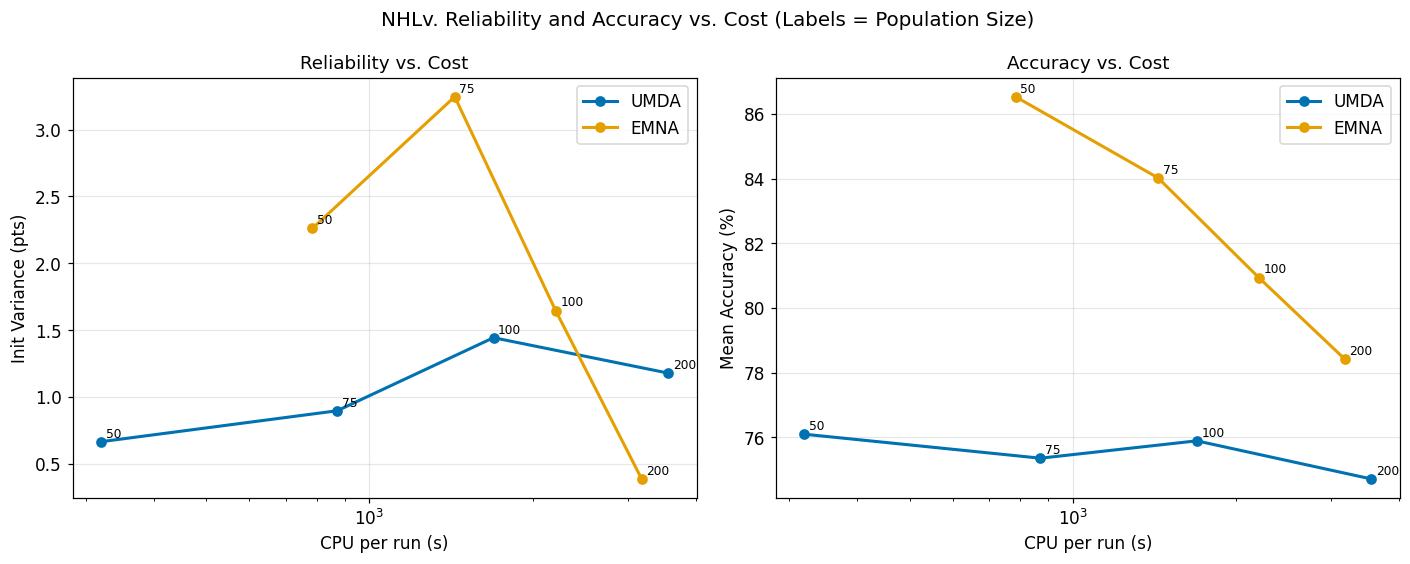
\includegraphics[width=\textwidth]{figures/43_pop_tradeoff_nhlv.png}
\caption{\emph{NHLy} (\texttt{utility\_only}, \texttt{binary}+\texttt{regret}): init
variance (left) and mean accuracy (right) against CPU cost per run, population labelling
each point.}
\label{fig:pop-tradeoff-nhlv}
\end{figure}

\begin{figure}[h!]
\centering
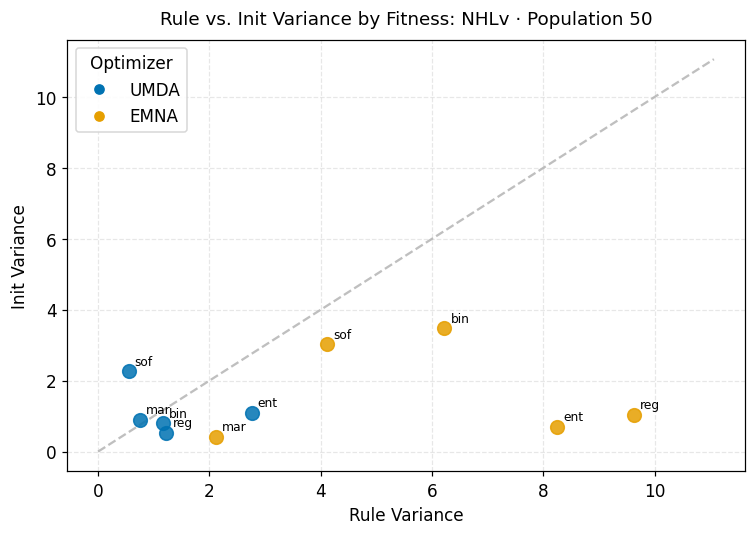
\includegraphics[width=0.55\textwidth]{figures/43_diag_nhlv.png}
\caption{\emph{NHLy} (\texttt{utility\_only}, population $50$): rule effect versus init
effect per fitness and optimizer.}
\label{fig:pop-diag-nhlv}
\end{figure}

\newpage
% ==============================================================
\section{First results}
\label{sec:stopmode-degeneracy}
% ==============================================================

Although the convergence study in Section~\ref{sec:stopmode} was conducted to determine the stopping criterion, it also provides the first relevant results of this chapter, detailed in Table~\ref{tab:stopmode-satisfiers}. A key finding is related to the satisfiers (individuals that reproduce the training rules \emph{perfectly}) because they exhibit completely different behavior in unseen scenarios. The convergence grids in Figures~\ref{fig:stopmode-bypass} and~\ref{fig:stopmode-nhlv1} demonstrate this progression across generations, where the gap between the ``best'' (green) and ``worst'' (red) individuals exemplifies this degeneracy. 

Exploring this variance represents a promising line of research: it would be highly beneficial to identify the minimal set of rules that yields maximum accuracy and which combination of them provides the greatest information gain. However, although analytical methods exist for this, the present thesis will assume that a domain expert already knows, or at least has a hint, based on experience, which specific subset of rules guarantees a high success rate.


\begin{table}[h!]
\centering
\small
\setlength{\tabcolsep}{5pt}
\begin{tabular}{ll|cccc|cccc}
\hline
 & & \multicolumn{4}{c|}{\textbf{mean accuracy (\%)}}
   & \multicolumn{4}{c}{\textbf{std (\%)}}\\
\textbf{net} & \textbf{opt}
 & \textbf{5} & \textbf{10} & \textbf{20} & \textbf{30}
 & \textbf{5} & \textbf{10} & \textbf{20} & \textbf{30}\\
\hline
bypass & UMDA & 54 & 59 & 64 & 71 & 3.8 & 3.6 & 2.9 & 4.6\\
       & EMNA & 54 & 59 & 64 & 73 & 4.6 & 5.2 & 5.9 & 6.5\\
       & EGNA & 56 & 63 & 64 & 71 & 3.5 & 5.6 & 3.5 & 5.4\\
       & KEDA & 73 & 73 & 77 & 81 & 4.6 & 5.0 & 7.1 & 7.2\\
\hline
NHLy   & EMNA & 81 & 80 & 89 & 94 & 2.2 & 2.1 & 6.6 & 6.3\\
       & UMDA & 73 & 75 & 79 & 83 & 1.9 & 2.5 & 2.7 & 3.6\\
\hline
\end{tabular}
\caption{Accuracy on different rule sets of the satisfiers (indiv. that reproduce every training rule), by network, optimizer and fraction of rules exposed ($5$--$30\%$), measured at the \texttt{top90} stopping point (Section~\ref{sec:stopmode-cost}). ``Mean'' is the satisfier accuracy
averaged over the repetitions; ``std'' is its standard deviation \emph{across} those repetitions. EGNA and KEDA
were run only on \emph{bypass}. On \emph{bypass} all optimizers use the $400$-individual population adopted in Section~\ref{sec:popsize}; \emph{NHLy} uses $50$.}
\label{tab:stopmode-satisfiers}
\end{table}

\subsection{Effect of the number of rules exposed}

This subsection analyses how the amount of supervision, i.e.\ the fraction of
rules shown to the search, affects the recovered policy. 

\begin{itemize}
    \item The first quantitative
result is that \textbf{the recovery is clearly beneficial}. On every network and optimizer the mean satisfier accuracy in
Table~\ref{tab:stopmode-satisfiers} stops well above the random baseline ($50\%$
on \emph{bypass}, $42\%$ on \emph{NHLy}) and climbs steadily as more rules are
exposed. Even the smallest budget helps, though modestly for the hardest optimizers: a
\emph{single} rule on \emph{bypass} ($5\%$ of the base) lifts the mean to
$54$--$73\%$ --- only a couple of points over the one-rule baseline
($52.5\% = \frac{50\%\times19 test+100\%\times1train}{20}$ on \textit{bypass}) for
UMDA/EMNA, but well above it for KEDA --- and richer budgets raise it into the
$71$--$94\%$ range. At the larger budgets, then, the recovery buys up to twenty-odd
accuracy points at no extra cost, merely through the application of EDAs.

 \item The second message is the other side of working with so few
rules: \emph{which} rule is drawn matters. Each repetition sees a different random rule subset, so the standard deviation in the table measures the sensitivity to that draw. It stays within a few points, but with a single rule a bad draw can still pull a run down to the baseline (notice that a rule will always contributes to improve the accuracy and if a run falls below the based line is only a matter of probability). 

\end{itemize}

The number is relevant, but also the quality of the rules that support the estimation of the parameters through the EDA, the generic rules, the exception cases, and the coverage of the problem; it is the expert who evaluates this aspect of quality.



\begin{figure}[h!]
\centering
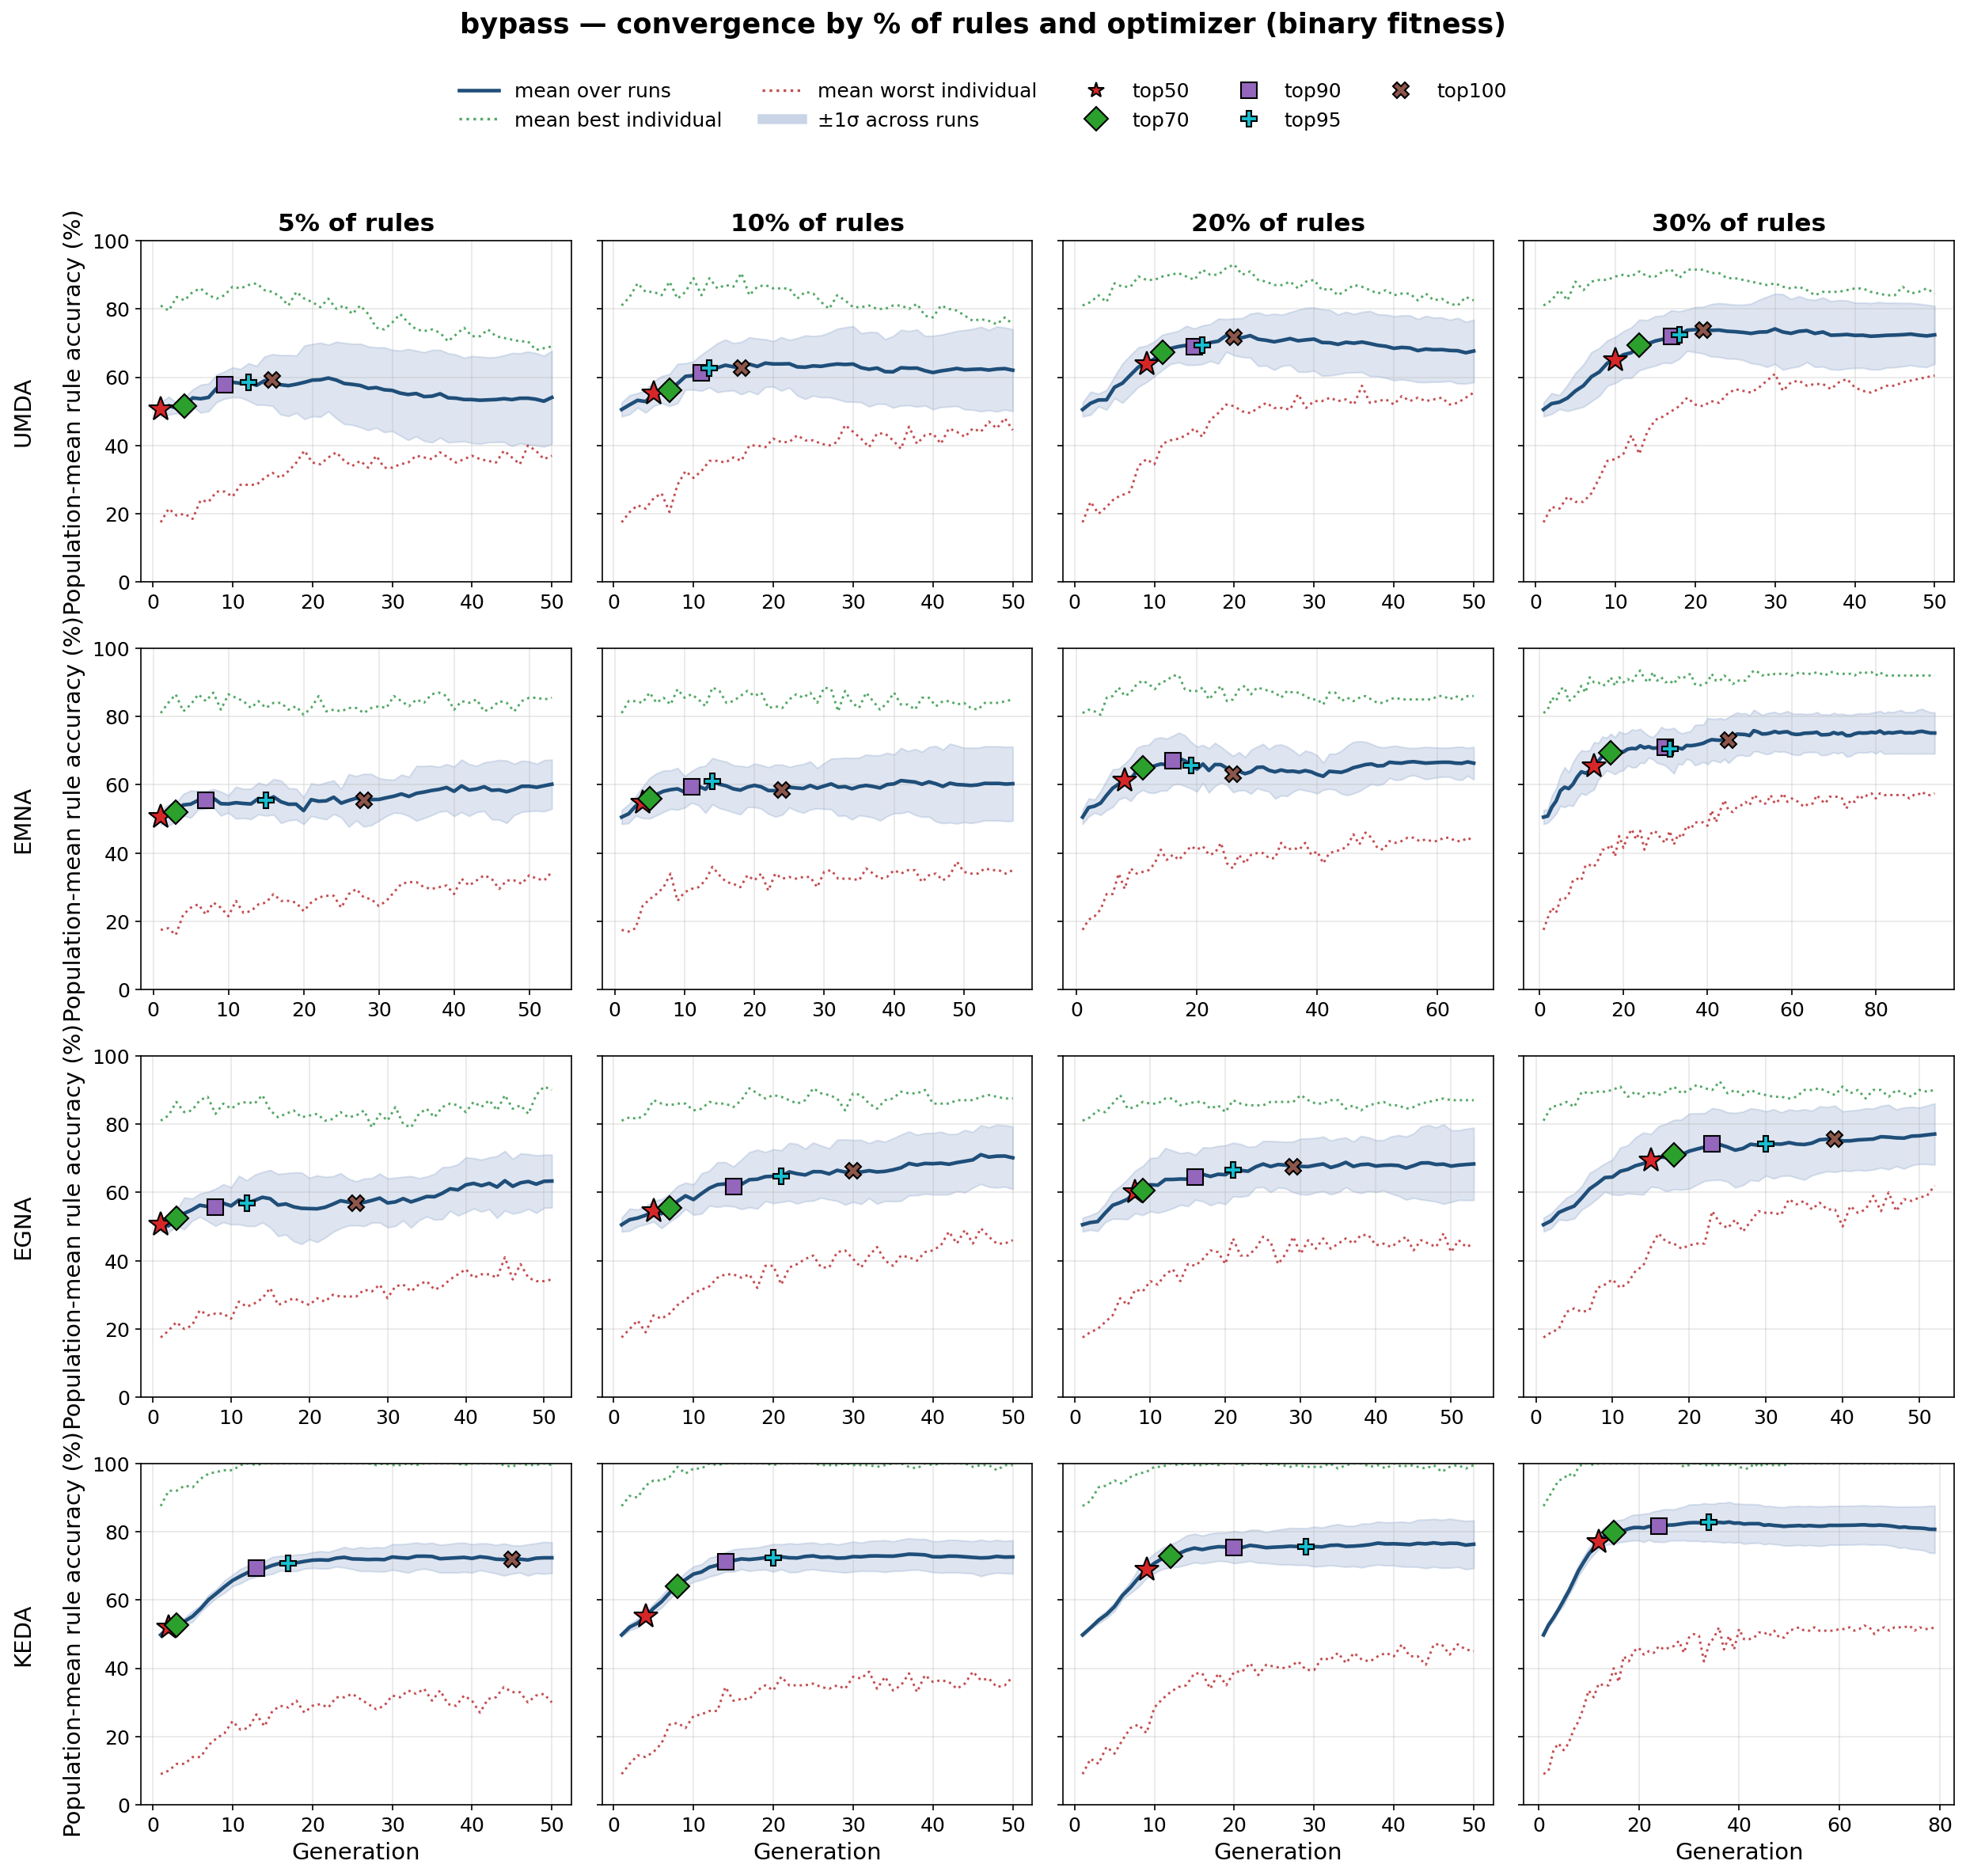
\includegraphics[width=\textwidth]{figures/stopmode_bypass_curves.png}
\caption{Convergence on \emph{bypass} by fraction of rules (columns) and
optimizer (rows: UMDA, EMNA, EGNA, KEDA), \texttt{binary} fitness. Solid: mean
population accuracy with a $\pm1\sigma$ band across repetitions; dotted: mean of
the best (green) and the worst (red) individual; markers: the
\texttt{top50}--\texttt{top100} transitions.}
\label{fig:stopmode-bypass}
\end{figure}


\begin{figure}[h!]
\centering
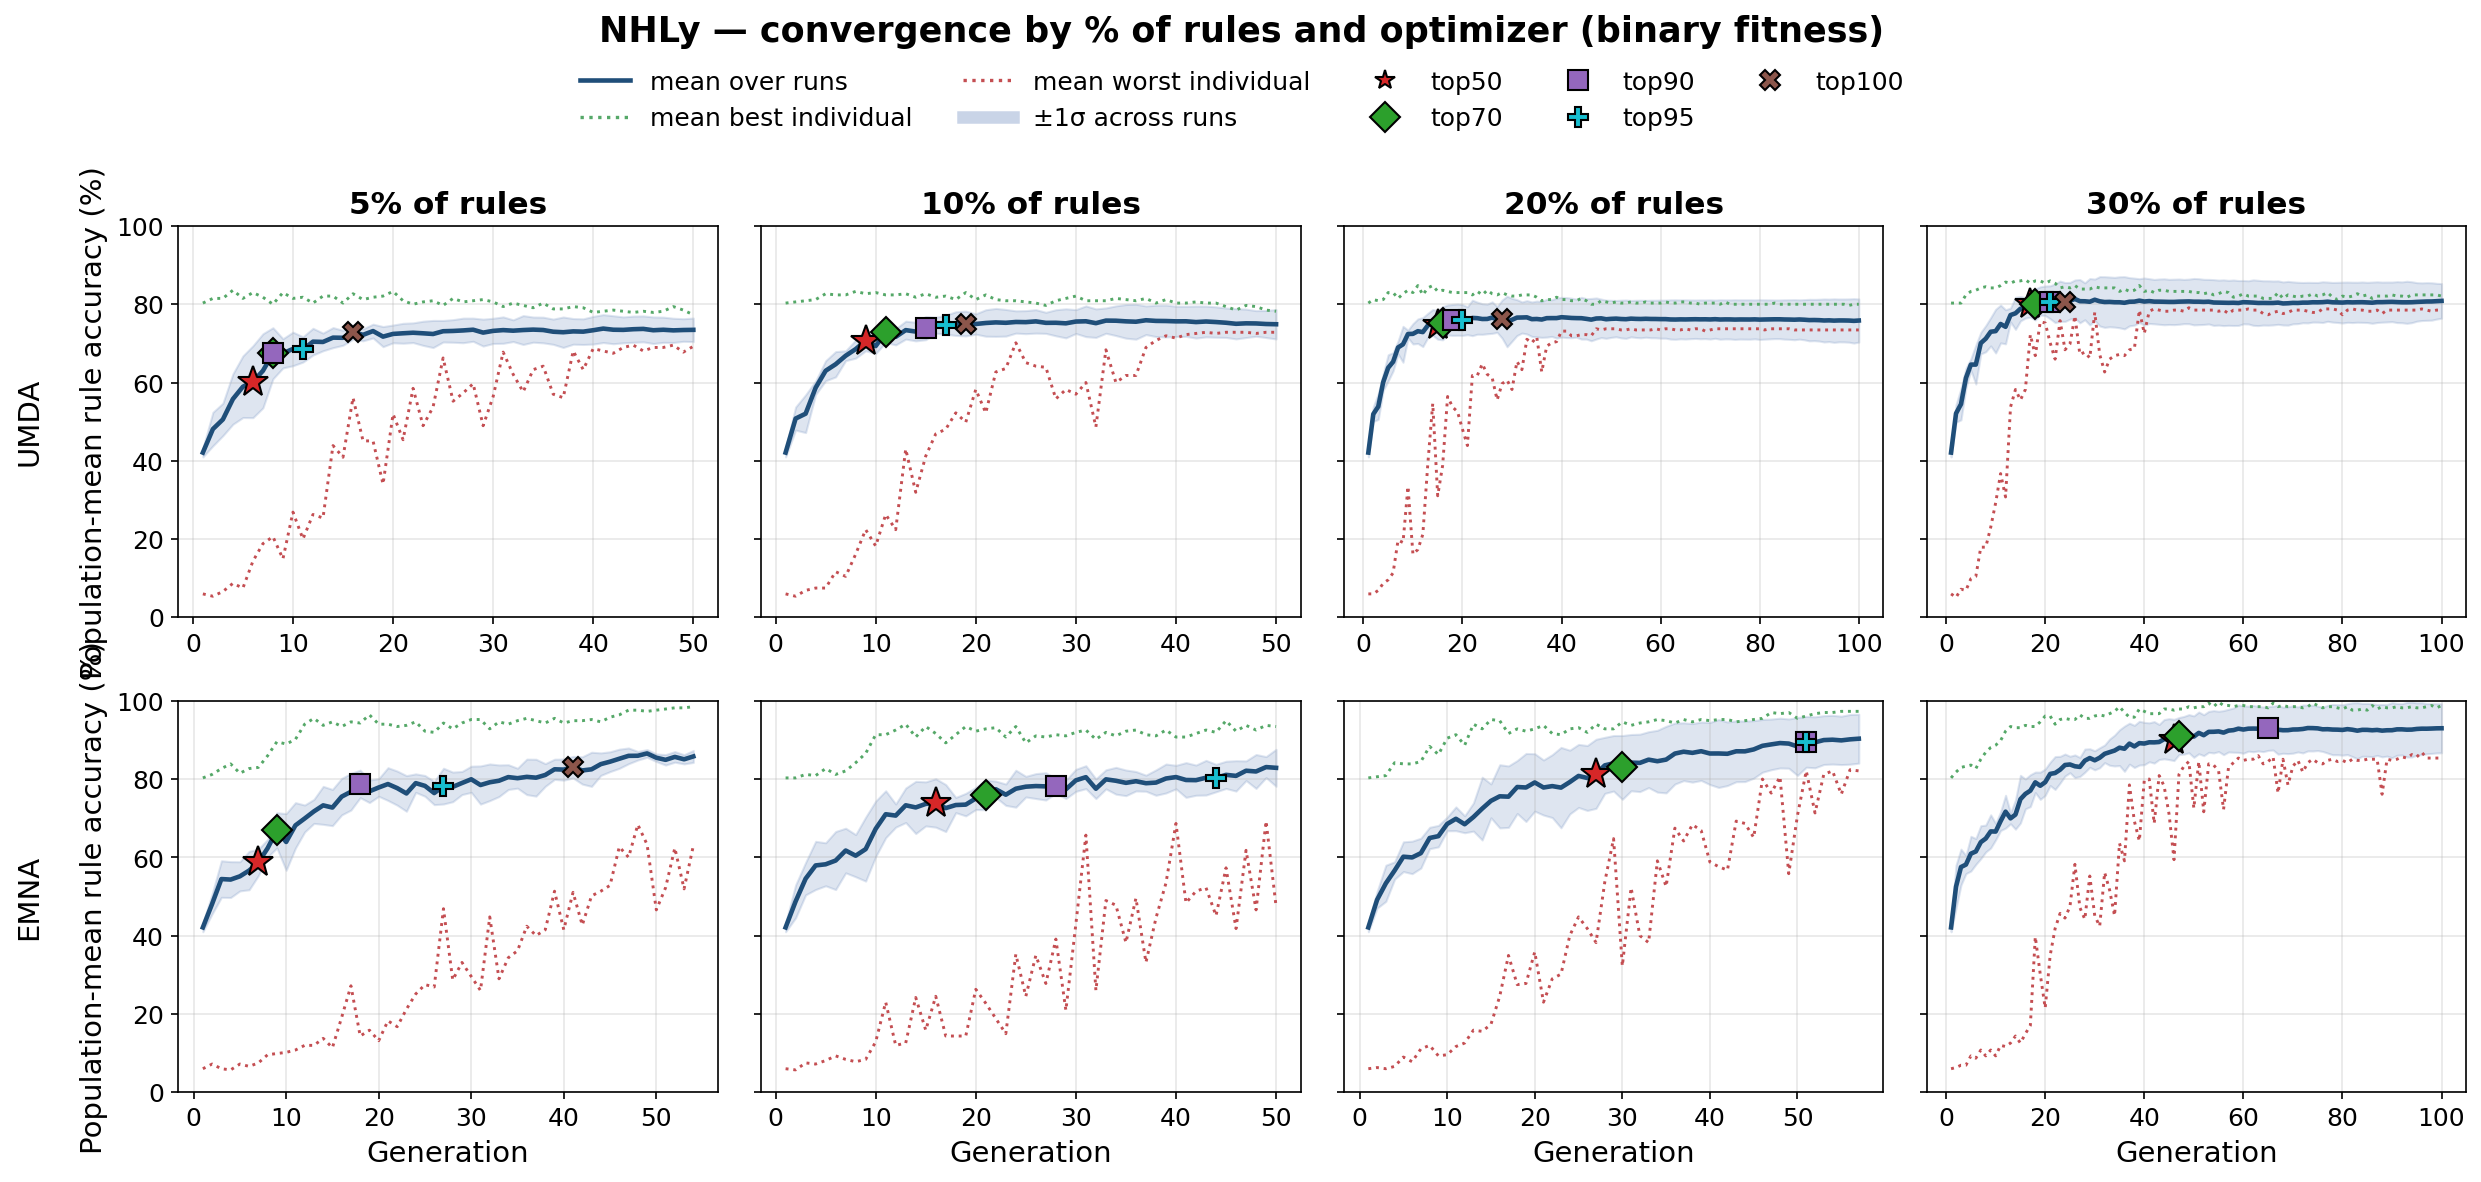
\includegraphics[width=\textwidth]{figures/stopmode_nhlv1_curves.png}
\caption{Convergence on \emph{NHLy} by fraction of rules (columns) and
optimizer (rows: UMDA, EMNA), \texttt{binary} fitness, \texttt{utility\_only}
mode. Conventions as in Figure~\ref{fig:stopmode-bypass}.}
\label{fig:stopmode-nhlv1}
\end{figure}

\subsection{The role of the optimizer}

The optimizers differ in the level they reach, in their robustness to the rule
drawn, and in their cost (Figure~\ref{fig:stopmode-bypass}). \textbf{KEDA is both
the strongest and the most robust} on \emph{bypass}: it reaches the highest mean
($69$--$81\%$) and the smallest sensitivity to the rule drawn (std $\le\!6$; even
its worst repetitions stay around $65\%$), not because of the population number
($400$ individuals have been also tried in UMDA and EMNA with t) but due to its kernel-density model that covers all the search space, finding better solutions.


\textbf{UMDA, EMNA and EGNA} reach a similar, lower level ($\sim\!55$--$76\%$). Cost, however, separates them on two
compounding counts. Per generation, UMDA and EMNA are about an order of magnitude
cheaper than EGNA and KEDA ($\sim\!0.05$ against $\sim\!0.55$ CPU seconds). And
the expensive pair also needs \emph{more} generations to reach \texttt{top90} and
stabilize (KEDA a median of $19$ generations against UMDA's $12$) so the
two factors multiply: reaching the stopping point costs about $0.5$~s with UMDA
or EMNA but $8$--$10$~s with EGNA or KEDA, a $15$--$20\times$ gap
(Figure~\ref{fig:cpu-top90}). This makes \textbf{EGNA the poorest in
cost--benefit}: as slow as KEDA, yet no more accurate than the cheap UMDA and
EMNA.


On \emph{NHLy} only the cheap pair is affordable: EGNA and KEDA are dropped, as
their per-run cost is prohibitive on a parameter vector this large (and KEDA's
kernel estimate degenerates under certain conditions).
Here the EMNA-versus-UMDA contrast becomes decisive
(Figure~\ref{fig:stopmode-nhlv1}).
\newpage

\textbf{EMNA clearly wins}: its mean climbs
from $81\%$ to $94\%$ as rules are added, whereas \textbf{UMDA} is limited in a
lower $73$--$83\%$ band (although both sit far above the $42\%$ baseline
and both are stable across rule draws, std $\lesssim 7$). The grid shows the reason
UMDA population collapses early into a tight but low
region, while EMNA keeps exploring until it reaches the high-accuracy one. That
extra accuracy is paid in convergence time, not in per-generation speed
(Figure~\ref{fig:cpu-top90}). At small-to-moderate budgets EMNA needs more
generations to reach \texttt{top90} (a median of $18$--$51$ against UMDA's
$8$--$19$) so its recovery costs roughly twice as much.

\begin{figure}[h]
\centering
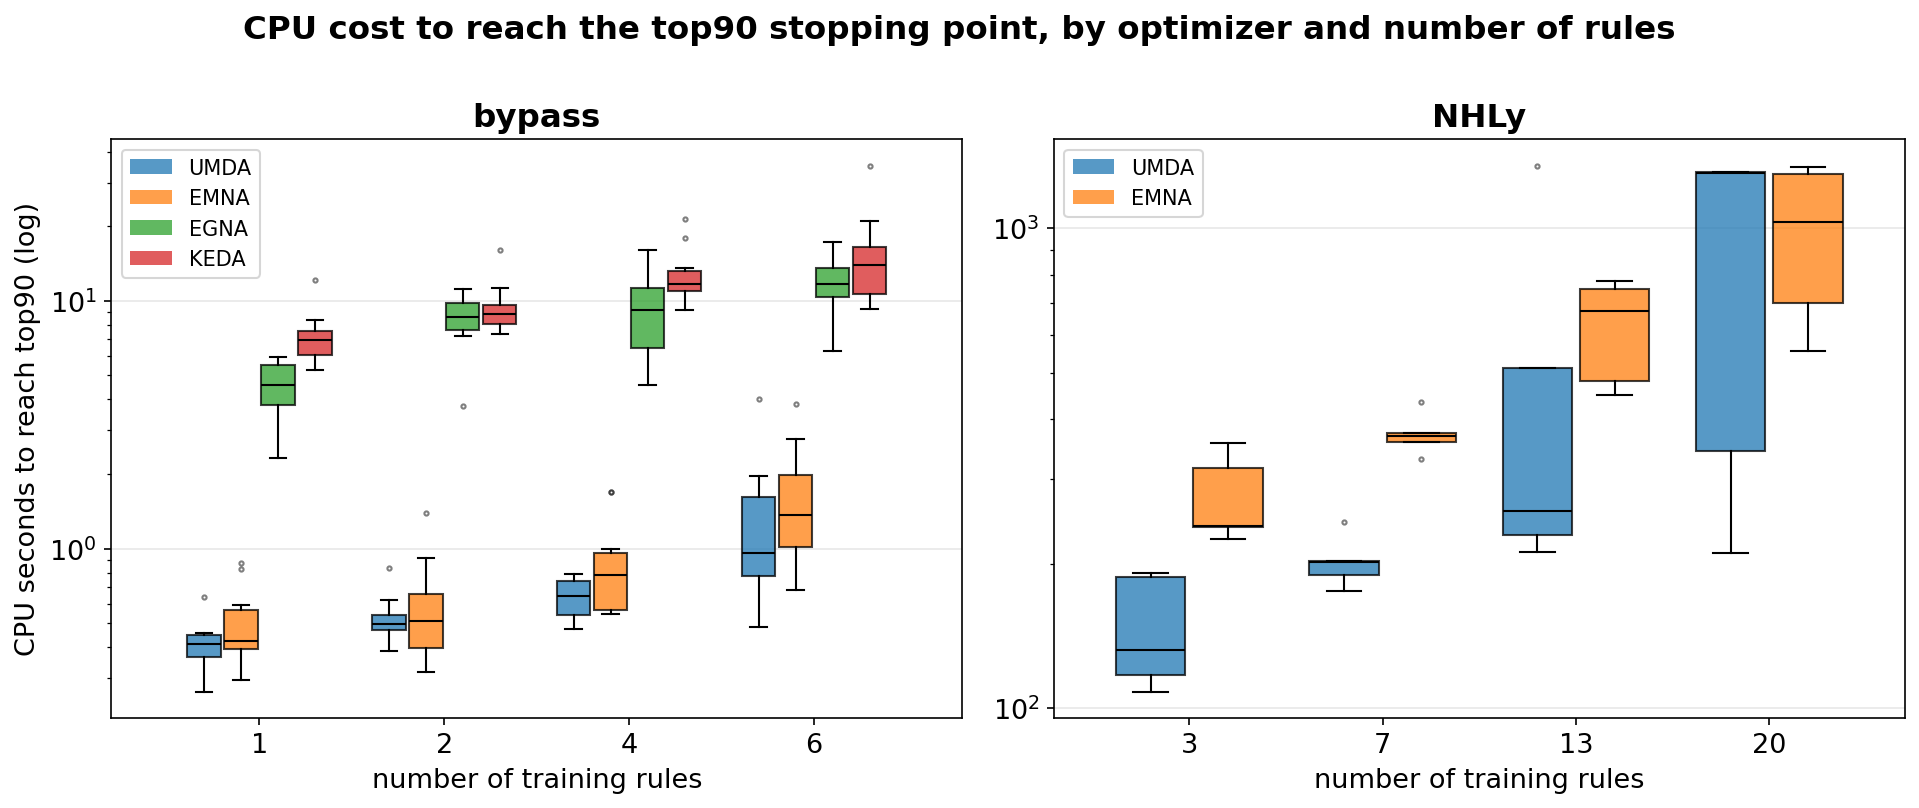
\includegraphics[width=\textwidth]{figures/stopmode_cpu_top90.png}
\caption{CPU seconds to reach the \texttt{top90} stopping point (per run,
logarithmic scale), by optimizer and number of training rules on the tho IDs.}
\label{fig:cpu-top90}
\end{figure}

\subsection{Convergence dynamics and what is worth recovering}
\label{sec:stopmode-markov}

Two contrasting trends emerge from the convergence grids (Figures~\ref{fig:stopmode-bypass} and~\ref{fig:stopmode-nhlv1}). Across repetitions, the $\pm1\sigma$ band \textbf{widens} (in the \emph{bypass} network at $30\%$ of the rules, it increases from $\sim\!2$ to $\sim\!6$--$10$ points before saturating). On the opposite, \emph{within} a single run, the gap between the best and worst individuals \textbf{narrows} (in \emph{NHLy}, decreasing from $\sim\!74$ to $\sim\!5$ points). Viewed as a Markov chain, each repetition represents an independent path that originates from a near-uniform model and drifts toward a \emph{distinct} satisfier optimum (Section~\ref{sec:stopmode-degeneracy}). 

The inter-run variance accumulates similar to a random walk, eventually plateauing at a width that reflects the extent of the degenerate subspace, while selective pressure continuously contracts each population toward its specific point of convergence. Consequently, the individual runs diverge from \emph{one another}, even as they become internally more homogeneous.

A final practical observation merits attention. In the \emph{bypass} configuration, the recovery process fits both the probability tables and the utilities (\texttt{both}), whereas in \emph{NHLy}, it only recovers the utilities (\texttt{utility\_only}). Despite its significantly larger size, \emph{NHLy} achieves higher accuracy ($\sim\!73$--$94\%$ compared to $\sim\!55$--$81\%$). This indicates that \textbf{attempting to recover the probabilities is detrimental rather than beneficial} (at least with this binary fitness function); the rules fail to identify them, and the introduction of extra free parameters merely expands an already degenerate search space.

We draw two primary conclusions from this study:
\begin{itemize}
  \item The stopping criterion behaves as a knee point characterized by
        decreasing returns, justifying our selection of \texttt{top90}.
  \item \emph{Reproducing the training rules is not equivalent to recovering the
        underlying policy.} The only reliable method to bridge this gap is to
        expose the system to a broader set of rules.
\end{itemize}

\newpage
% ==============================================================
\section{Comparing the loss functions}
\label{sec:fitness}
% ==============================================================

While the convergence study (Section~\ref{sec:stopmode}) established \emph{when} a run should stop, and the population study (Section~\ref{sec:popsize}) determined the appropriate number of individuals, this section evaluates the impact of using different loss functions for the recovery process. We compare the five loss variants introduced in Section~\ref{sec:losses} across two main configurations. The first is the \emph{bypass} case in the joint \texttt{both} mode (population of $400$, $20\%$ of the rules exposed), and the second is the \emph{NHLy} case in \texttt{utility\_only} mode (population of $50$). For both setups, we perform five independent repetitions per loss function and optimizer. We evaluate each recovery based on its mean population accuracy and CPU time. Ultimately, the goal is to determine whether a smoother, more informative loss function recovers the policy more effectively than the plain \texttt{binary} baseline, or if the added complexity yields no tangible benefit.

\subsection{Bypass}
\label{sec:fitness-bypass}

On \emph{bypass} the five losses are \textbf{interchangeable in accuracy}
(Table~\ref{tab:fitness-bypass}): the spread across losses and optimizers is
smaller than spread over the repetition. The smoother landscape the continuous and likelihood losses promise does not translate into a
better recovered policy.

\begin{table}[h!]
\centering
\begin{tabular}{lccc}
\toprule
 & \multicolumn{2}{c}{\textbf{acc\_mean (\%)}} & \textbf{gens.}\\
\textbf{loss} & UMDA & EMNA & (range)\\
\midrule
\texttt{binary}  & $66$ & $63$ & $6$--$16$\\
\texttt{regret}  & $65$ & $65$ & $5$--$16$\\
\texttt{margin}  & $67$ & $66$ & $19$--$24$\\
\texttt{softmax} & $66$ & $64$ & $9$--$15$\\
\texttt{entropy} & $66$ & $68$ & $9$--$15$\\
\bottomrule
\end{tabular}
\caption{\emph{Bypass}, \texttt{both} mode, population $400$, $20\%$ of the rules, five repetitions. ``acc\_mean'' is the mean population accuracy per
optimizer; ``gens.'' the range of stopping generations across the two optimizers.
}
\label{tab:fitness-bypass}
\end{table}

Because the accuracies coincide, the choice falls to secondary qualities. Here the
losses do differ: \texttt{binary} and \texttt{regret} converge fastest and
\texttt{margin} slowest, and \texttt{binary} is also the simplest and cheapest to
evaluate. As accurate as any, among the quickest to converge, and the least
complex, \texttt{binary} is the natural baseline on this network.

\subsection{NHLy}
\label{sec:fitness-nhlv}

The results on the larger \emph{NHLy} dataset, demonstrate that the choice of loss function becomes decisive when the search space requires a more active guidance (Table~\ref{tab:fitness-nhlv}). Furthermore, performance is highly tied to the optimizer: the continuous, utility-aware \texttt{regret} loss clearly maximizes EMNA's capabilities, reaching a peak accuracy of $89.7\%$, followed by the \texttt{binary} baseline at $83.9\%$. The remaining losses fail to provide an advantage for EMNA. Conversely, UMDA is unable to exploit any of the loss formulations; as noted in Section~\ref{sec:stopmode-degeneracy}, it collapses early and stagnates between $75\%$ and $78\%$ regardless of the chosen metric.

\begin{table}[h!]
\centering
\begin{tabular}{lcc}
\toprule
\textbf{loss} & \textbf{UMDA} & \textbf{EMNA}\\
\midrule
\texttt{regret}  & $75.1$ & $\mathbf{89.7}$\\
\texttt{binary}  & $75.2$ & $83.9$\\
\texttt{entropy} & $77.4$ & $78.7$\\
\texttt{softmax} & $78.1$ & $77.5$\\
\texttt{margin}  & $76.4$ & $77.5$\\
\bottomrule
\end{tabular}
\caption{\emph{NHLy}, \texttt{utility\_only}, population $50$, $10\%$ of the rules,
mean population accuracy (\%) averaged over repetitions.}
\label{tab:fitness-nhlv}
\end{table}


\subsection{The utility temperature shapes the recovery}
\label{sec:fitness-temperature}

To control the effect that the decoding of the parameter vector may have on the loss space across the different fitness functions, we sweep across five utility temperature ($T_u$) values. In essence, this temperature modifies the utility values to either smooth or accentuate the resulting utility distribution. This effect can soften or sharpen the optimization landscape, preventing the search from saturating prematurely or getting trapped in suboptimal regions.

To isolate its effect, we fix the true CPTs and recover only the utilities on the \emph{bypass} configuration (\texttt{utility\_only}, population $400$), sweeping $T_u$ across a geometric range centered around $1$. Figure~\ref{fig:utemp-heat} illustrates the recovery performance (both in terms of final accuracy and convergence speed) across the different losses. 

Two clear, monotonic trends emerge, specifically for the stricter \texttt{binary} and \texttt{regret} losses. As $T_u$ increases, it simultaneously \textbf{improves the mean accuracy} (e.g., \texttt{binary} climbs from $\sim\!95\%$ at $T_u=0.25$ to $\sim\!97\%$ at $T_u=4$) and \textbf{speeds up convergence} (the required generations drop from $5.1$ to $3.8$).   Note that we removed \texttt{margin} from the speed heatmap because it never satisfied the stopping criterion and consistently hit the $50$-generation cap, so it is omitted from the convergence plot to preserve the color scale for the others.

\begin{figure}[h!]
\centering
\includegraphics[width=\textwidth]{figures/bypass_utemp_heat.png}
\caption{\emph{Bypass}, \texttt{utility\_only}, population $400$, $20\%$ of the
rules, averaged over the two optimizers and repetitions. Left: mean population
accuracy over the loss $\times\,T_u$ grid; right: mean generations to reach the
\texttt{top90} stopping point.}
\label{fig:utemp-heat}
\end{figure}

The reason follows directly from how the parameters are decoded
(Section~\ref{sec:encoding}): each utility is the sigmoid $\sigma(\phi/T_u)$ of a
raw searched value, so $T_u$ sets the steepness of that squashing (sharp and
saturating at low $T_u$, quasi-linear at high $T_u$). What is specific to this
experiment is the effect of that steepness on an \emph{EDA}, which samples a whole
population of raw vectors around its current estimate. At a low $T_u$ the
saturation makes each decision fragile and instable: near a boundary an infinitesimal change of the raw vector flips the decoded utility between extremes and the search needs more generations to settle. At
a high $T_u$ the squashing is gentle, the same population spread leaves the
decisions unchanged, the population decodes to near-identical policies, and the
smoother landscape is reached sooner. 

A low $T_u$ saturates the decoded utilities to extreme values, which impacts each loss differently. This is our interpretation :

\begin{itemize}
    \item \textbf{\texttt{regret}:} As a magnitude-based loss, it relies on continuous gradients. Under a low $T_u$, the utility gap collapses to either $0$ or the maximum range, degenerating into a scaled \texttt{binary} loss. A higher $T_u$ keeps the utilities graded and restores this gradient, which is why \texttt{regret} benefits the most.
    \item \textbf{\texttt{binary}:} This loss only evaluates the $\arg\max$ and, unlike the others, has no built-in mechanism to keep utilities away from extreme values. It is completely exposed to saturation. A higher $T_u$ acts as a gentler decoder, pulling the utilities back into a graded, well-separated regime, which explains its improvement on \emph{bypass}.
\end{itemize}

Meanwhile, \texttt{margin}, \texttt{softmax}, and \texttt{entropy} already sit at their accuracy ceiling in this scenario, leaving no room for further improvement.

However, these results may be specific to \emph{bypass}. On a network with a different geometry the balance could well invert: the extreme utilities that a low $T_u$ produces are
also a way of sweeping the utility space more aggressively, and a harder problem
(where the search must travel further to separate the actions) might benefit
from that wider exploration rather than be penalized for it.
\newpage
% ==============================================================
\section{A few rules recover most of the policy}
\label{sec:saturation}
% ==============================================================

A recovery keeps improving as more rules are shown
(Section~\ref{sec:stopmode-degeneracy}); this section asks the natural question
``\emph{how many is enough}''. We measure it with the following experiment: for
each rule budget $k$ we launch an \emph{independent} recovery that is shown
exactly $k$ true rules and let it \emph{run to convergence}; the resulting model is
then scored against the \emph{whole} policy. Sweeping $k$ traces how far the
recovery reaches as a function of how many rules it is given (each $k$ a fresh
run). On \emph{bypass} we sweep $k=1,2,\dots,20$ one rule at a time (three
repetitions, each with a different set of training rules and its own
initialization) at the $400$-individual population fixed in
Section~\ref{sec:popsize}, in \texttt{both} mode (recovering the chance tables
\emph{and} the utilities) and with each of the two
fitness functions, \texttt{binary} and \texttt{regret}. 

Crucially, and unlike the
earlier sections, each run is now let converge rather than stopped early: it runs
for a minimum of $20$ generations (or earlier if \emph{all} of the population
reproduce the rules, \texttt{top100}) and then stops as soon as the best $90\%$ do
(\texttt{top90}), capped at $100$ generations. The minimum matters because, when a high fraction of the rules is used for training, the \texttt{top90} criterion is met too quickly (gen. 1 or 2) and, on its own, would halt the search before the model has had time to reach accuracies close to $100\%$. On the much larger
\emph{NHLy}, where each recovery is far more expensive, we sweep $k=3,6,\dots,21$
in steps of three, with three repetitions, the \texttt{regret} loss stopped at
\texttt{top70} (here we do not reach high fraction of rules during training so we can use a looser criterion), in \texttt{utility\_only} mode. Both networks use UMDA and EMNA.

\begin{figure}[h!]
\centering
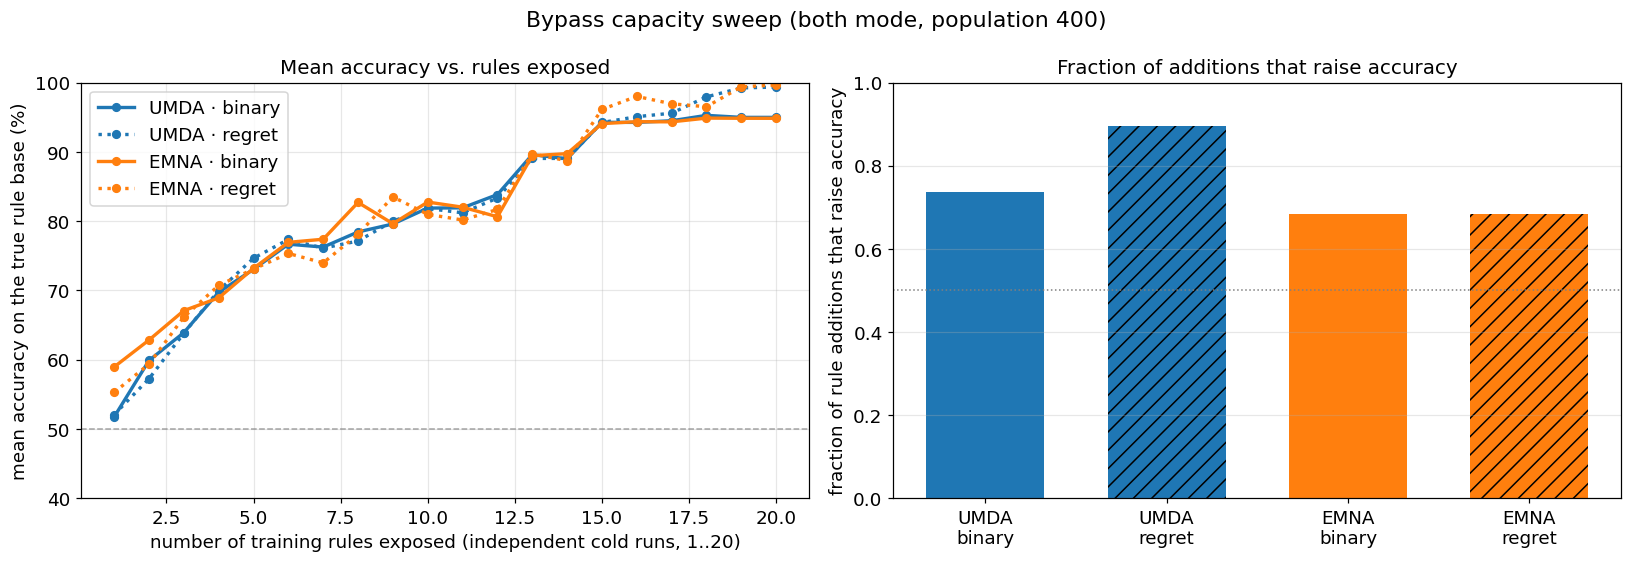
\includegraphics[width=\textwidth]{figures/saturation_bypass_both.png}
\caption{\emph{Bypass} (\texttt{both} mode, population $400$, min.\ $20$
generations then \texttt{top90}): capacity sweep over the number of exposed rules
($k=1,\dots,20$, independent recoveries, three repetitions), with
\texttt{binary} (solid) and \texttt{regret} (dotted). Left: mean accuracy on the
true rule base against the number of rules exposed. Right: the fraction of
one-rule additions that raise accuracy.}
\label{fig:saturation}
\end{figure}


Two things emerge on \emph{bypass} (Figure~\ref{fig:saturation}). First, the recovery gain is \textbf{clearly non-linear} with respect to the number of rules. An untrained model averages $\sim\!50\%$ (pure chance on the binary decisions) and a \emph{single} rule barely moves it ($\sim\!52\%$ for UMDA, $\sim\!59\%$ for EMNA): one constraint is far too little to pin the whole diagram. From there, the curve grows steeply as the first handful of rules buy the most. Accuracy climbs to $\sim\!73\%$ by five rules and $\sim\!82\%$ by ten, capturing roughly two-thirds of the total gain. After this rapid initial growth, the curve bends and flattens out, demonstrating that achieving $100\%$ compliance requires observing a very high percentage of the total rules.

Second, the picture \textbf{barely depends on the loss or the optimizer}. UMDA and
EMNA track each other almost exactly across the sweep (EMNA is only ahead at the
very first rules: $59$ vs $52\%$ at $k=1$) because \emph{bypass} is small
enough for the independent-marginal model of UMDA to capture. The loss separates them
only at the very end: \texttt{regret} pins the policy more completely, closing to
$\sim\!100\%$ at twenty rules, while \texttt{binary} plateaus around $95\%$ (\texttt{top100} is not achieved within the 20 generations in \textit{bypass}). Here \textbf{most added rules do help}: the fraction of
one-rule additions that raise accuracy stays well above one half for every
configuration ($0.68$--$0.89$; Figure~\ref{fig:saturation}, right).


That parity breaks on the larger network (Figure~\ref{fig:saturation-nhlv}).
\textbf{EMNA converts rules into accuracy far better than UMDA}: it climbs steadily
from $\sim\!64\%$ at three rules to $\sim\!95\%$ at twenty-one, while UMDA does more slowly and reaches around $79\%$
(the same result seen in Section~\ref{sec:stopmode-degeneracy}).
Note also that here the coarse addition helps that the addition of three rules per step results useful. Each jump carries enough new
signal that the accuracy keeps rising monotonically across the whole sweep except in only one case.


\begin{figure}[h!]
\centering
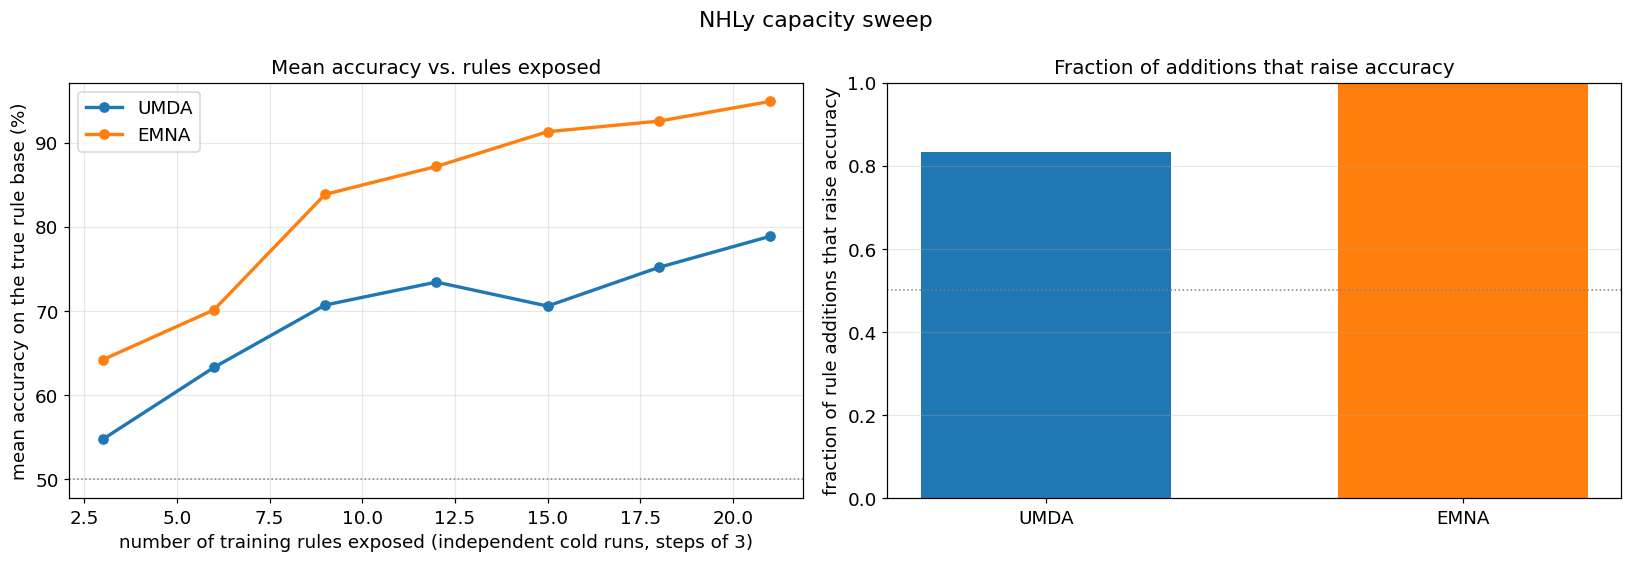
\includegraphics[width=\textwidth]{figures/saturation_nhlv.png}
\caption{\emph{NHLy}: the same capacity sweep on the larger network, coarser
($k=3,6,\dots,21$ in steps of three, three repetitions). Left: EMNA converts rules
into accuracy steadily up to $\sim\!95\%$ while UMDA lags and tops out lower.
Right: at three rules per step every addition helps ($100\%$ for both optimizers),
so the accuracy rises monotonically across the sweep.}
\label{fig:saturation-nhlv}
\end{figure}

The first few rules buy the largest
gains, lifting the policy well above chance, while each further rule pays diminishing
returns, and the last points up to full recovery are the expensive ones that need
almost the whole rule base. Identifying \emph{which} small set of rules is most informative rather than simply adding more.

\newpage
% ==============================================================
\section{Decisive rules matter more than their number}
\label{sec:greedy}
% ==============================================================

Section~\ref{sec:saturation} showed that the first few rules capture most of the
accuracy, but left open whether \emph{which} specific rules are chosen actually matters. 
This section investigates exactly that: instead of adding
\emph{random} rules, we \textbf{search greedily} for highly informative ones and 
subsequently analyze what distinguishes a good rule set from a poor one. Starting from a single seed
rule, at each step we evaluate \emph{every} remaining rule as the next potential addition. We train
each candidate set to \texttt{top90} (\texttt{binary} loss, \texttt{both} mode on \emph{bypass}),
and retain the one yielding the highest accuracy on the true $20$-rule base
(using a majority vote of the satisfiers, as in Section~\ref{sec:stopmode-cost}). We grow
this set until isolating the best \emph{eight} rules. 

To prevent bias from a single lucky seed, we
repeated the entire procedure across three distinct initial rules and network initializations (these three \emph{chains} are seeded here by rules $14$, $3$, and $0$) using both UMDA and EMNA. 
Consequently, at every step, we record not just the greedy winner but
the accuracy of \emph{all} other candidates, capturing the full distribution of how
much the ``next'' rule matters.

\subsection{The composition matters as much as the count}
\label{sec:greedy-spread}

The central finding is that \textbf{for a fixed initial rule, the specific choice of the complementary rules leads to a wide dispersion in accuracy} (Figures~\ref{fig:greedy-c0}--\ref{fig:greedy-c2}). At \emph{every} step, the performance gap between the best and worst candidates drastically exceeds the median gain of adding a new rule (a massive spread of $\sim\!20$--$35$ points versus a median advance of just $\sim\!4$ points). Put differently, a single well-chosen rule is worth several mediocre ones.

The greedy path climbs steadily to $90$--$95\%$ but \emph{saturates around five to six rules}. Beyond this, new additions yield negligible gains, perfectly mirroring the diminishing returns established in Section~\ref{sec:saturation}. Conversely, the worst choice at each step stagnates near the initial baseline. This proves that counting rules is only half the story; \emph{composition} is the other half. Finally, both optimizers agree on this overall trajectory, with EMNA only lagging briefly at initialization due to noisier full-covariance sampling before catching up entirely by the third rule.

\begin{figure}[h!]
\centering
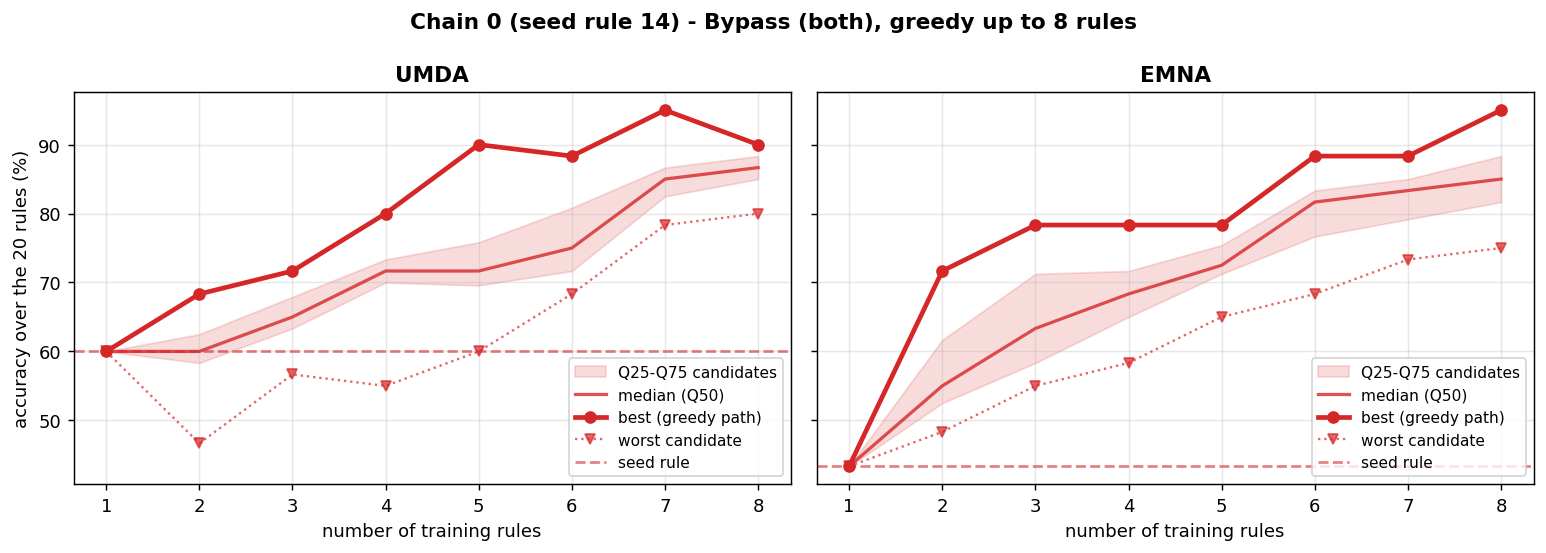
\includegraphics[width=\textwidth]{figures/48_cadena0.png}
\caption{\emph{Chain 0} (seed rule $14$), \emph{bypass} (\texttt{both}): accuracy
vs.\ number of training rules, UMDA (left) and EMNA (right). Band is the
Q25--Q75 spread over \emph{all} candidate rules at each step; the thick line is the
greedy winner (best candidate), the dotted line the worst, and the dashed
horizontal line the accuracy of the single seed rule.}
\label{fig:greedy-c0}
\end{figure}

\begin{figure}[h!]
\centering
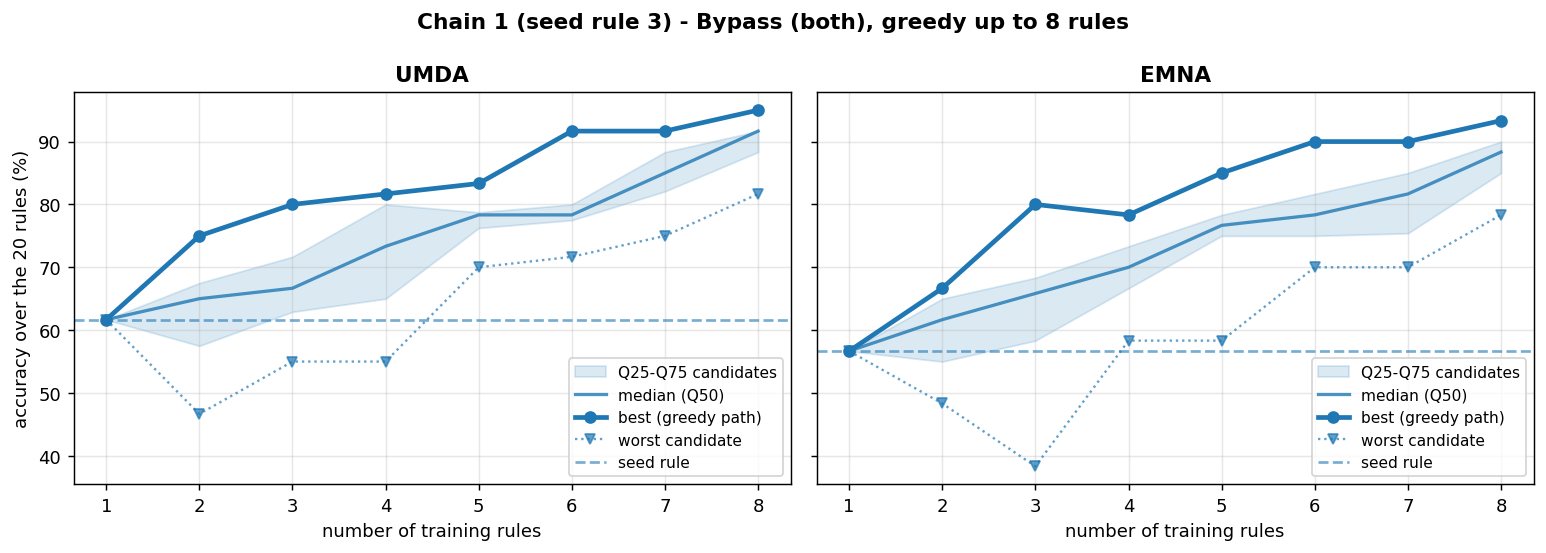
\includegraphics[width=\textwidth]{figures/48_cadena1.png}
\caption{\emph{Chain 1} (seed rule $3$), \emph{bypass} (\texttt{both}). Same
layout as Figure~\ref{fig:greedy-c0}.}
\label{fig:greedy-c1}
\end{figure}

\begin{figure}[h!]
\centering
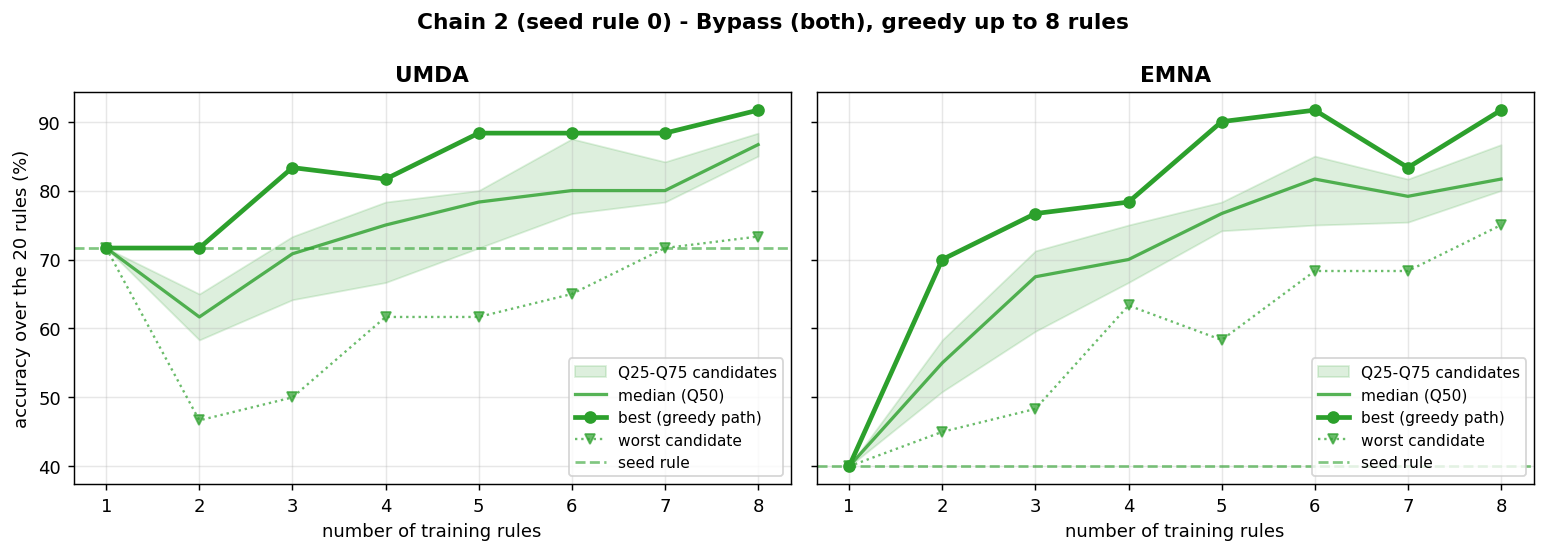
\includegraphics[width=\textwidth]{figures/48_cadena2.png}
\caption{\emph{Chain 2} (seed rule $0$), \emph{bypass} (\texttt{both}). Same
layout as Figure~\ref{fig:greedy-c0}.}
\label{fig:greedy-c2}
\end{figure}

Crucially, the choice of rule dictates far more than just accuracy: it drives also a great variance in both \textbf{convergence cost} (CPU time) and \textbf{probability-table MSE} (Figure~\ref{fig:greedy-cost}). For instance, at a fixed rule count, training time can swing by more than four times purely based on \emph{which} rule is added. 

Furthermore, these costs are essentially \emph{correlated} with accuracy ($|\rho|\!\lesssim\!0.15$). This implies that a poorly chosen rule is a double threat: it can be simultaneously less accurate and slower to converge. Despite this variance, the probability-table error remains consistently small throughout. This confirms the decoupling between accuracy and probability-table reconstruction: accuracy improves by rearranging the policy encoded by the utilities, not by reconstructing the original CPTs.

\begin{figure}[h!]
\centering
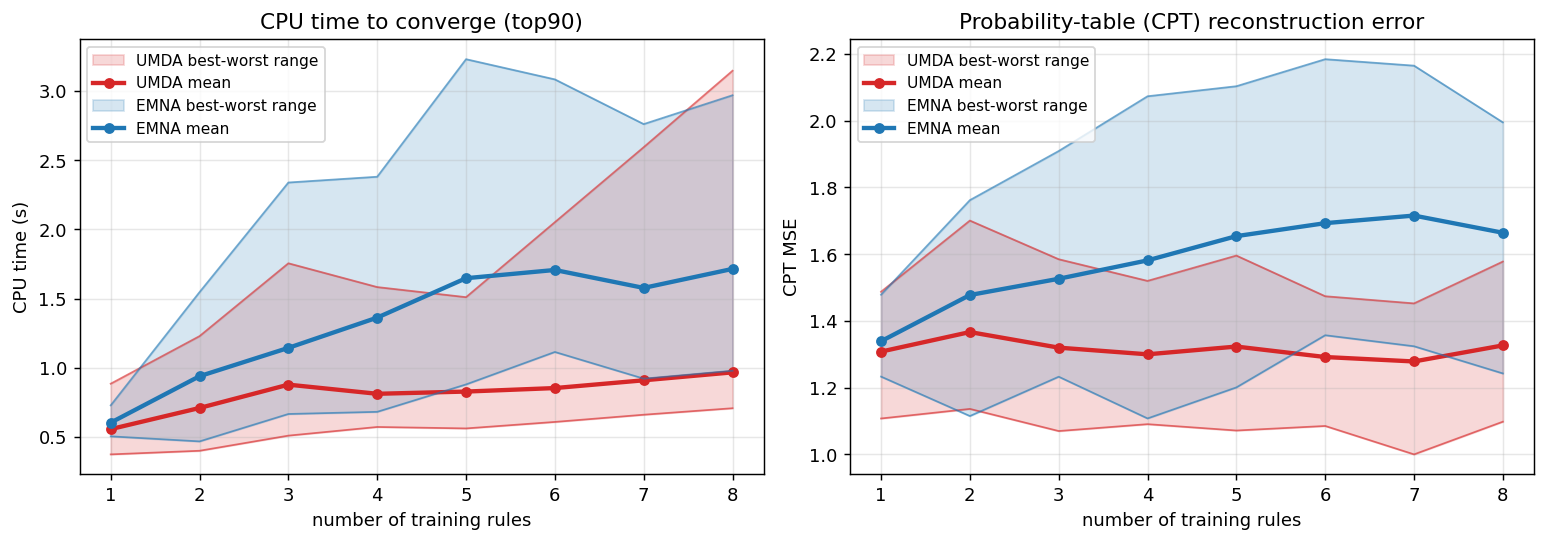
\includegraphics[width=\textwidth]{figures/48_mse_cost.png}
\caption{\emph{Bypass} (\texttt{both}): best--worst \textbf{spread} over all
candidate rules at each rule count (band between the fastest/lowest and
slowest/highest candidate), aggregated over the three chains. UMDA in red, EMNA in
blue. Left: CPU time to \texttt{top90}; right: probability-table (CPT)
reconstruction error.}
\label{fig:greedy-cost}
\end{figure}

\newpage
\subsection{Decisive rules make the good sets}
\label{sec:greedy-patterns}

When mastering a medical domain, an expert intuitively internalizes the most critical, high-stakes decisions before addressing marginal or highly specific exceptions. We can quantify this learning hierarchy using a rule's \emph{utility gap}: the expected-utility difference between the optimal action and its closest alternative, $\lvert EU(\text{optimal})-EU(\text{alternative})\rvert$. In the \emph{bypass} model, which chains two binary decisions (whether to medicate, \texttt{HEARTPHARMA}, and whether to operate, \texttt{HEARTSURGERY}), the wider this gap, the more decisively the scenario dictates the overall policy. 

This is precisely the notion of informativeness that grounds regret-based utility elicitation: in the minimax-regret framework of Boutilier et al.~\cite{boutilier2006minimax,braziunas2007minimax}, the queries that most reduce uncertainty about the utility function are those with the largest utility gap, whereas near-tie scenarios (where every action yields almost the same expected utility) reveal little about the underlying preferences. We therefore advance the following \textbf{hypothesis}: a rule's utility gap is closely related to how strongly it drives the recovered policy, so that decisive, high-gap rules tend to be more informative than near-indifferent ones.

To probe this hypothesis we reuse the rule sets recovered in the previous experiment (\texttt{both} mode, population~$400$, \texttt{binary} loss, \texttt{top90}). From each of the three recovery groups we take the five highest-accuracy chains (fifteen rule sets in total) and count, for every rule, how many of these fifteen best sets contain it, discarding the first rule of each chain since it is drawn at random. Because the two decision nodes operate on very different utility scales (surgery triggers larger swings than medication), we keep them apart and plot each rule's appearance count against its utility gap, separated by decision node (Figure~\ref{fig:perrule-margin}). 

A correlation emerges between how often a rule appears among the highest-accuracy chains and its utility gap. In \texttt{HEARTSURGERY}, the appearance count climbs steeply with the gap: the two decisive rules ($16$, $18$) dominate the best sets while the two near-indifferent ones ($17$, $19$) never appear. In \texttt{HEARTPHARMA}, where the sixteen rules are narrowly clustered ($0.09$ to $0.46$), the relationship is weaker, yet the most frequently selected rules still tend to sit at the larger gaps.

\begin{figure}[h!]
\centering
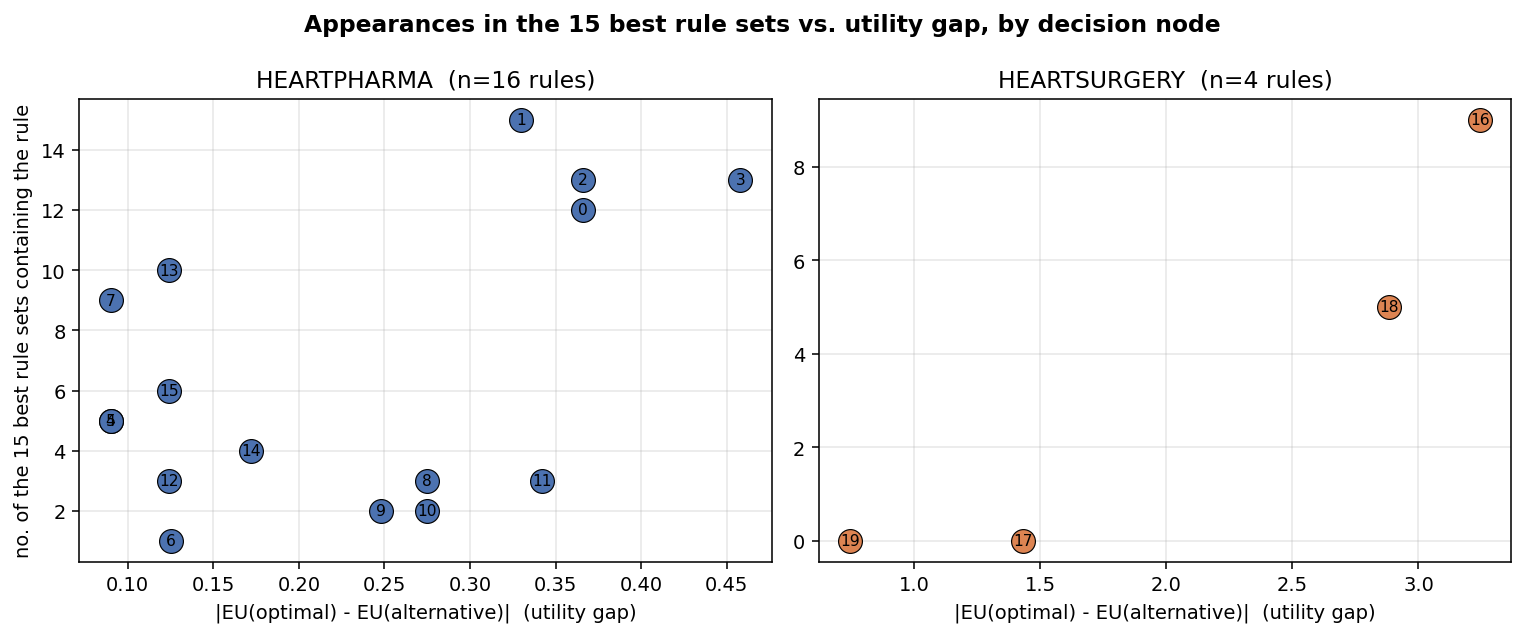
\includegraphics[width=\textwidth]{figures/58_freq_vs_margin.png}
\caption{Appearances in the fifteen best rul\emph{bypass} (\texttt{both},population~$400$), split by decision node. Each point is a rule, placed at its utility gap $\lvert EU(\text{optimal})-EU(\text{alternative})\rvert$; its height is the number of the fifteen highest-accuracy chains (the five best from each of the three recovery groups) that contain it, excluding the randomly chosen first rule of each chain. In the surgery node, where the gaps are widely dispersed, the decisive high-gap rules appear far more often; in the tightly clustered medication node the relationship is much weaker.}
\label{fig:perrule-margin}
\end{figure}





% ==============================================================
\section{The Dominance of Utilities over Probabilities}
\label{sec:loss}
% ==============================================================
As our final experiment, we now examine what the recovery process actually captures. The most straightforward test is to isolate each component of the model by fixing the other to its true value. We either search solely for the utilities (\texttt{utility\_only}) or solely for the conditional probability tables (CPTs) (\texttt{chance\_only}, while recording the CPT reconstruction error, the MSE), and then compare these isolated searches to a joint recovery of \emph{both} components. Every run in this section uses the five loss functions, five initializations and five rule sets, at $20\%$ of the rules and with the \texttt{top90} stopping rule. Our primary finding is that the utilities dictate the overall behavior: the policy is inherently driven by the utility matrix.

Figure~\ref{fig:recovery} (left) illustrates the result of the each recovery. Searching exclusively for the utilities reproduces the policy with near perfection ($\sim\!96\%$ for both optimizers), whereas searching solely for the CPTs yields a much lower accuracy ($\sim\!66\%$). By itself, this might not seem surprising, as the number of utility parameters is significantly lower than the number of parameters representing the CPTs. 

Interestingly, however, recovering both components simultaneously (despite the increase in the total number of parameters) yields an accuracy comparable to, or even higher than, the \texttt{chance\_only} baseline ($\sim\!68\%$). This is further corroborated by our observations in Section~\ref{sec:stopmode-degeneracy}: attempting to jointly recover probabilities and utilities in the \emph{bypass} model results in lower accuracies than recovering a larger model like \emph{NHLy} using only utilities, even though the parameter vector of the latter is less than half the size (64 versus 144, respectively, Table \ref{tab:benchmark-sizes}).

This counter-intuitive result can be explained by the degree of degeneracy inherent to each problem formulation. When probabilities are introduced as unknowns in the search space, degeneracy increases drastically due to the dense interdependencies among CPTs (an issue that barely affects utilities). This creates numerous degenerate solutions that satisfy the training rules but fail to generalize to all rules. At the same time, if only the CPTs are recovered while the utilities are kept fixed, the CPTs are forced to adjust erratically and drastically to fit those predefined utility values, resulting in slower and worse convergence (as demonstrated in our experiments). Conversely, if both CPTs and utilities are recovered, they can vary and mutually adapt at the same time, leading to a much more successful recovery of both seen and unseen rules.

Furthermore, accurately reproducing the decision rules does not guarantee a precise recovery of the CPTs. Across all \texttt{chance\_only} runs, rule accuracy is \textbf{uncorrelated} with the CPTs reconstruction error (Figure~\ref{fig:recovery}, right; Spearman $\rho\simeq0$). This indicates that a better alignment with the expert's rules does not necessarily translate into an improved estimation of the probability tables. As said, many other valid solutions with high rule accuracy appear.

Ultimately, we conclude that this discrepancy arises because the probability recovery problem is inherently more degenerate and complex than estimating the utilities. However, it should be noted that this has only been observed for the \emph{bypass} case, and we cannot guarantee that it will always hold true universally.

\begin{figure}[h!]
\centering
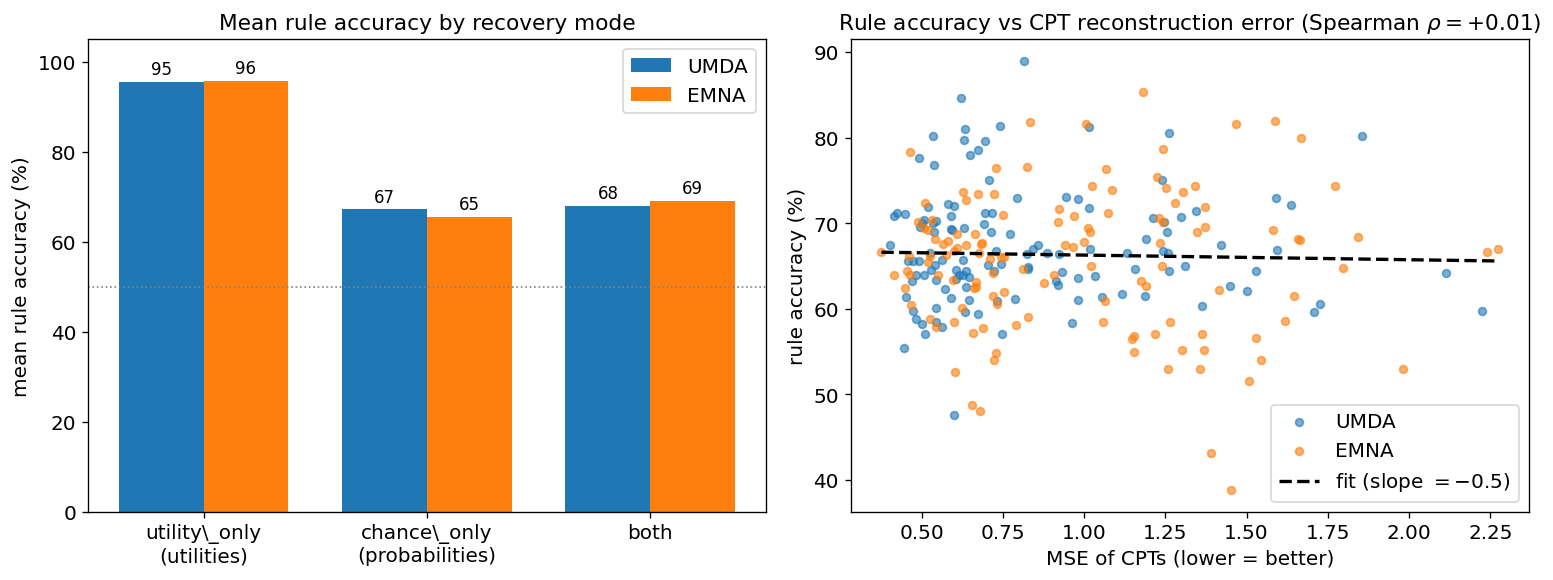
\includegraphics[width=\textwidth]{figures/59_recovery.png}
\caption{\emph{Bypass} ($20\%$ of the rules). Left: mean rule accuracy when
recovering only the utilities, only the probabilities, or both. Right: across all \texttt{chance\_only} runs the
accuracy is uncorrelated with the CPT-MSE.}
\label{fig:recovery}
\end{figure}





